\chapter{การวิเคราะห์และออกแบบระบบ}

การวิเคราะห์และออกแบบระบบก่อนดำเนินการจริงเป็นอีกหนึ่งขั้นตอนที่มีความสำคัญมาก เพราะการวิเคราะห์และออกแบบระบบนั้นเป็นการกระทำที่ทำให้ผู้พัฒนาเห็นรายละเอียดส่วนย่อยของงานทั้งหมด เพิ่มประสิทธิภาพในการวางแผน การทำงาน และยังช่วยลดปัญหาที่อาจจะเกิดขึ้นในระหว่างพัฒนา เพื่อให้ระบบมีความสมบูรณ์มากยิ่งขึ้น เนื่องจากการวิเคราะห์และออกแบบระบบนั้นจะช่วยให้ให้บริการ จัดการทรัพยากรได้อย่างคุ้มค่าและตรงตามความต้องการของระบบ

การวิเคราะห์และออกแบบแอปพลิเคชันสแกนอาหาร ในบทนี้จะแบ่งออกเป็น 6 ข้นตอนเพื่อให้เห็นการดำเนินงานอย่างมีระบบ ในหัวข้อแรกจะนำเสนอภาพรวมของระบบ ก่อนจะนำเสนอเอกสารแสดงความต้องการของระบบซึ่งจะทำให้เห็นที่มาของเพจต่าง ๆ ในขั้นตอนของการออกแบบในหัวข้อที่สาม ส่วนหัวข้อที่เหลือจะแสดงแผนภาพการการทำงานของระบบโดยใช้ UML diagram ซึ่งประกอบไปด้วย Use Case, Class และ Sequence Diagram เพื่อแสดงรายละเอียดของระบบก่อนนำไปเขียนคำสั่งด้วยภาษาโปรแกรมในบทต่อไป

\begin{enumerate}[label=3.\arabic*]
	\item โครงสร้างภาพรวมของระบบ (System Architecture) เป็นการออกแบบภาพรวมและเทคโนโลยีของระบบ
	\item System Requirements คือ ความต้องการหรือสิ่งที่ระบบควรจะทำ หรือหน้าที่หลักของ
	ระบบที่จะต้องทำ
	\item User Interface Design เป็นการออกแบบส่วนต่อประสานกับผู้ใช้
	\item Use Case Diagram เป็นแผนภาพที่ใช้แสดงให้ทราบว่าระบบทำงานหรือมีหน้าที่ใดบ้าง
	\item Class Diagram เป็นแผนภาพที่ใช้แสดง Class และความสัมพันธ์ระหว่าง Class
	\item Sequence Diagram เป็นแผนภาพที่ใช้แสดงให้เห็นถึงการตอบโต้ข้อมูลระหว่างคลาส เรียงตามลำดับของเวลาที่เกิดเหตุการณ์จากน้อยไปมาก
\end{enumerate}	

\section{รายละเอียดการออกแบบระบบ}
 ระบบแอปพลิเคชันสแกนอาหาร มีโครงสร้างการทำงานดังรูปที่ 3.1
   	\begin{figure}[H]
   		\centering
   		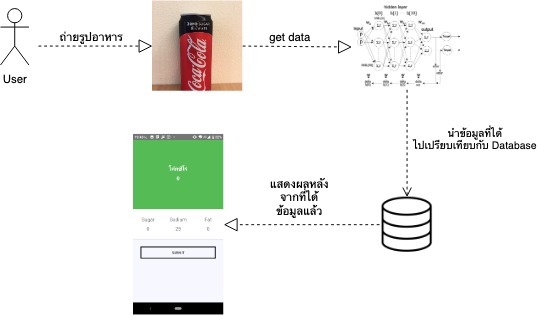
\includegraphics[width=\textwidth]{Figures/3/architecture/Arc1.jpg}
   		\caption{โครงสร้างการทำงานข้อระบบ}
   		\label{Fig:architecture}
   	\end{figure}
   
	 จากรูปที่ \ref{Fig:architecture} สามารถอธิบายโครงสร้างการทำงานของระบบได้ดังนี้ ผู้ใช้งานต้องทำการถ่ายภาพอาหารที่ต้องการ ระบบจะนำค่าที่ได้จากการถ่ายภาพไปเปรียบเทียบกับข้อมูลที่มีอยู่ใน
	 Database จากนั้นระบบจะทำการดึงข้อมูลที่มีอยู่มาแสดงผลเพื่อให้ผู้ใช้สามารถนำไปใช้งานต่อได้ 
   

\section{System Requirements}
\subsection{Functional Requirements} 
แอปพลิเคชันสแกนอหาร แบ่งตามประเภทผู้ใช้งานดังนี้ 
\begin{enumerate}
		\item ผู้ใช้งาน
			\begin{itemize}[label={--}]
				\item สามารถทำการเข้าสู่ระบบได้
				\item สามารถสแกนอาหารได้
				\item สามารถจัดการแอคเคาท์ของตนเองได้
				\item สามารถดูข้อมูลการบริโภคในรูปแบบวันได้
				\item สามารถดูข้อมูลการบริโภคย้อนหลังในรูปแบบสัปดาห์และเดือนได้ 
				\item สามารถเพิ่มอาหารที่ไม่มีอยู่ในระบบได้
			\end{itemize}
			\end{enumerate}

\subsection{Non-functional Requirements}
		\begin{enumerate}
		\item แอนดรอยด์แอปพลิเคชัน
		\begin{itemize}[label={--}]
			\item  แอปพลิเคชันสามารถดึงข้อมูลจาก Database ได้ภายในระยะเวลา 3 วินาที 
			\item  รองรับอาหารที่ผู้ใช้เพิ่มเข้ามาอย่างน้อย 500 ข้อมูล
			\item รองรับการใช้งานของผู้ใช้พร้อมกันอย่างน้อย 100 คน
		\end{itemize}
	\end{enumerate}
	
\section{User Interface Design}
ในการออกแบบ User Interface Design ของแอปพลิเคชันสแกนอาหาร ออกแบบมาให้มีลักษณะเสมือนจริงมากที่สุด โดยสามารถโต้ตอบกับผู้ใช้ได้ 
\item การออกแบบหน้าจอเข้าสู่ระบบ

				\begin{figure}[H]
					\centering
					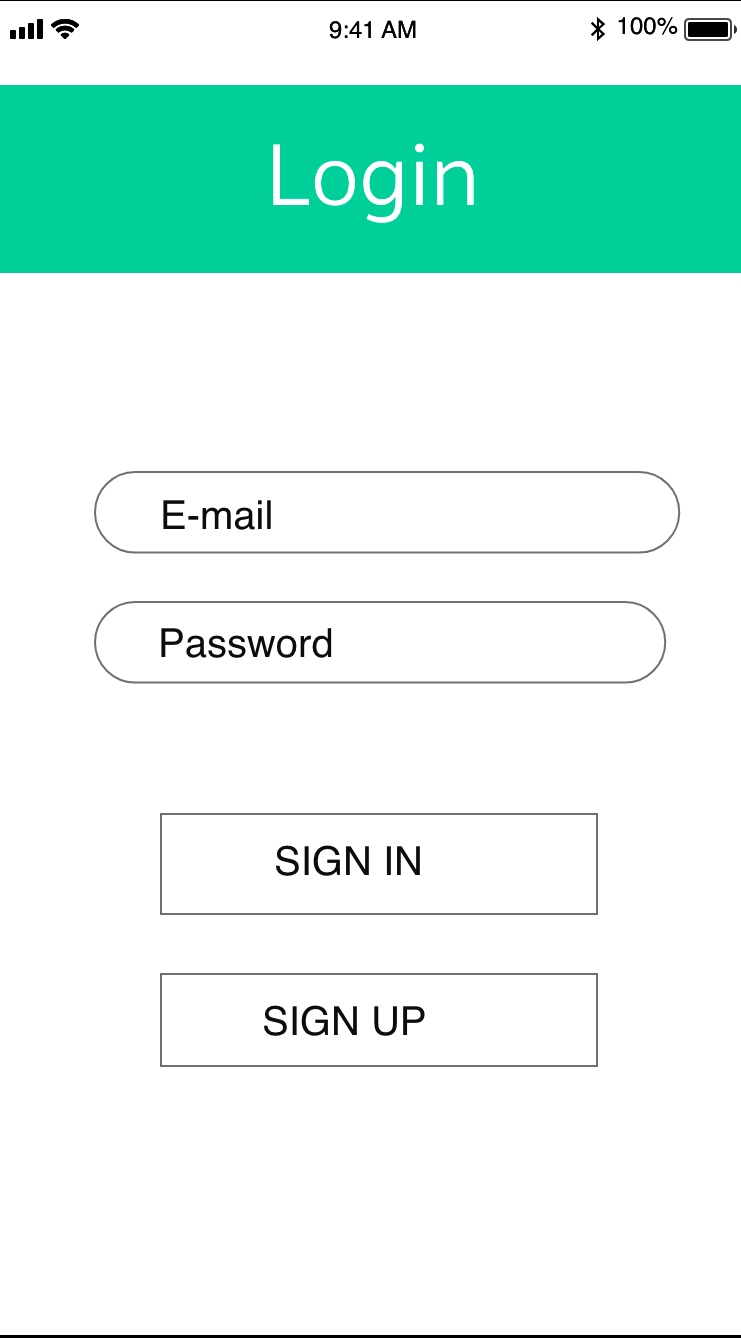
\includegraphics[width=0.2\textwidth]{Figures/3/UIDESIGN/1}
					\caption{หน้าจอ เข้าสู่ระบบ}
					\label{Fig:1}
				\end{figure}
				จากภาพที่ \ref{Fig:1} แสดงหน้าจอ เข้าสู่ระบบ เมื่อผู้ใช้ทำการติดตั้งแอปพลิเคชันครั้งแรก ระบบจะแสดงหน้านี้ขึ้นมาเพื่อให้ผู้ใช้ทำการสมัตรสมาชิกและเข้าสู่ระบบ
				หน้าจอเข้าสู่ระบบจะแสดงเพียงครั้งเดียวหากผู้ใช้เข้าสู่ระบบแล้วจะไม่มีการแสดงหน้าจอนี้ขึ้นมาอีก จนกว่าผู้ใช้จะทำการออกจากระบบ
\item การออกแบบหน้าจอสมัครสมาชิก 
	\begin{figure}[H]
					\centering
					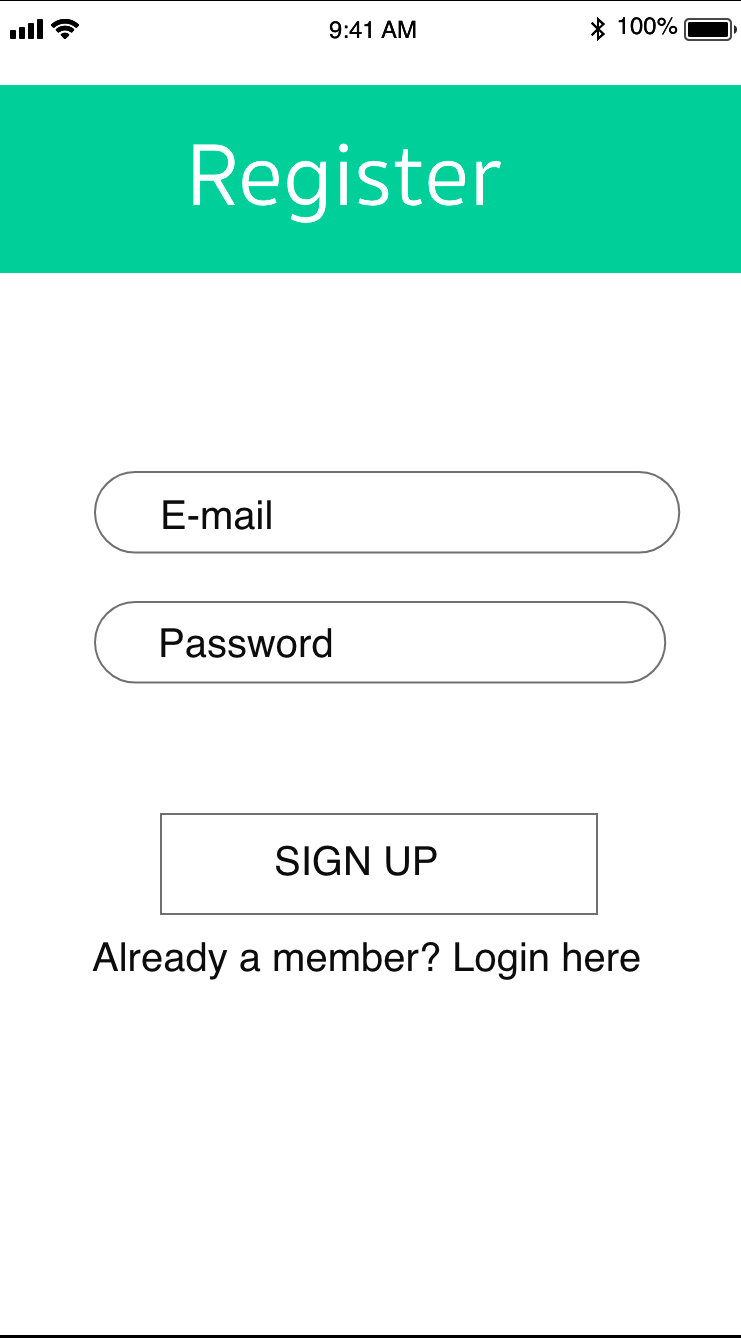
\includegraphics[width=0.2\textwidth]{Figures/3/UIDESIGN/2}
					\caption{หน้าจอ สมัครสมาชิก}
					\label{Fig:2}
				\end{figure}
				จากภาพที่ \ref{Fig:2} เมื่อผู้ใช้ทำการกดที่ปุ่ม SIGN UP ระบบจะทำการแสดงหน้าจอสมัครสมาชิกขึ้นมา ผู้ใช้จะต้องทำการใส่ Email address และ Password สำหรับการสมัครสมาชิกเมื่อ
				ใส่ข้อมูลครบแล้วทำการกดปุ่ม SIGN UP ในหน้าสมัครสมาชิก ก็จะเป็นการสมัครสมาชิกและเข้าสู่ระบบ
\item การออกแบบหน้าจอหลัก 
				\begin{figure}[H]
								\centering
								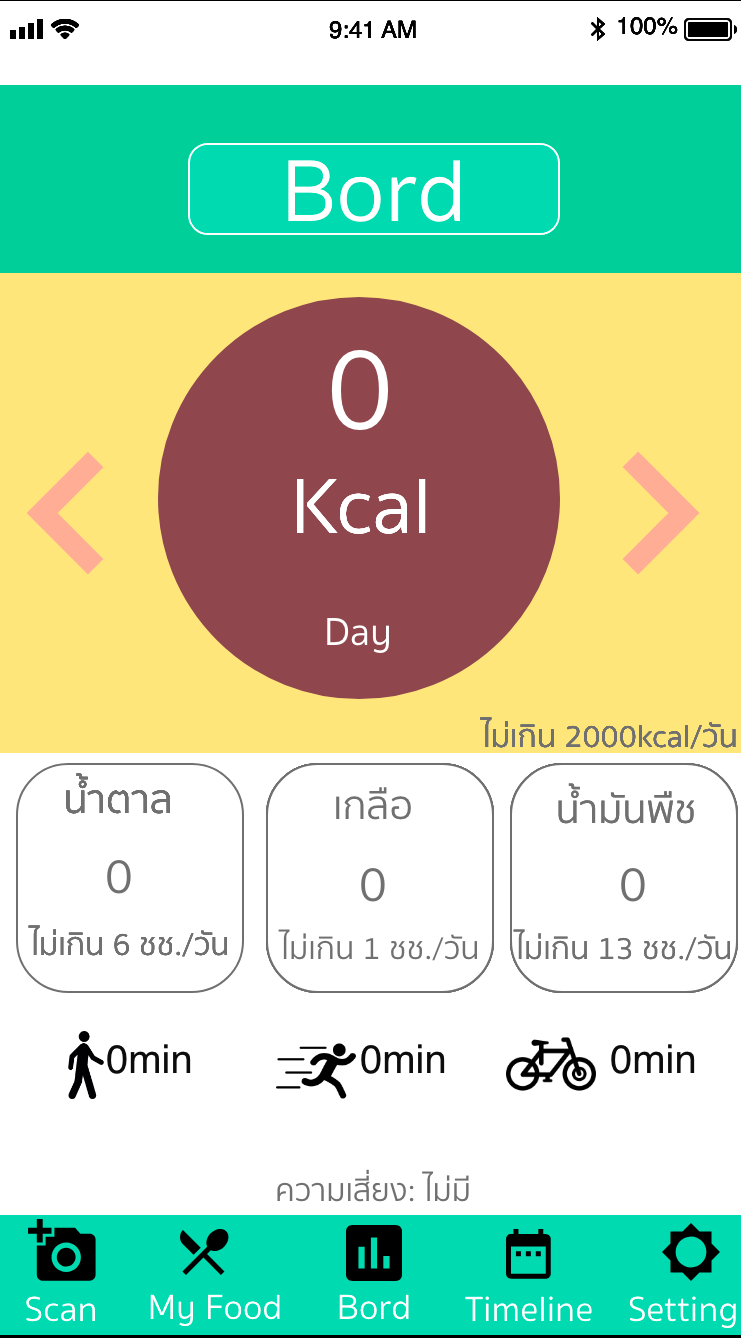
\includegraphics[width=0.2\textwidth]{Figures/3/UIDESIGN/5}
								\caption{หน้าจอ แดชบอร์ด}
								\label{Fig:5}
							\end{figure}
							จากภาพที่ \ref{Fig:5} หน้าแดชบอร์ด จะเป็นหน้าจอแรกที่แสดงหลังทำการเข้าสู่ระบบผู้ใช้สามารถดูข้อมูลสรุปรายวัน สัปดาห์และเดือน ได้และผู้ใช้สามารถไปยังหน้าจออื่นๆได้ผ่านหน้าจอหแดชบอร์ดนี้
\item การออกแบบหน้าจอสแกนอาหาร
				\begin{figure}[H]
								\centering
								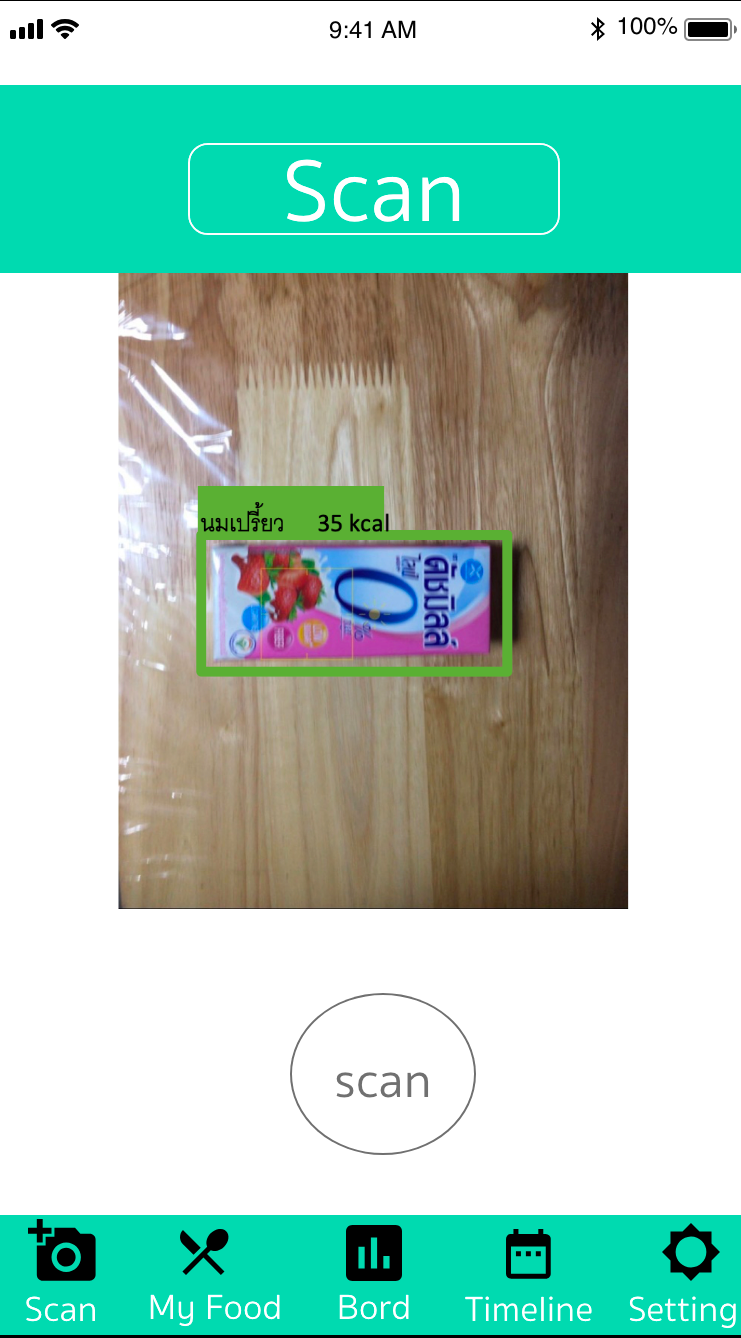
\includegraphics[width=0.2\textwidth]{Figures/3/UIDESIGN/4}
								\caption{หน้าจอ สแกนอาหาร}
								\label{Fig:4}
							\end{figure}
							จากภาพที่ \ref{Fig:4} ในหน้าจอสแกนอาหาผู้ใช้สามารถทำการกดที่ปุ่มสแกน โดยให้วัตถุที่ต้องการสแกนอยู่ในกรอบของกล้อง หลังจากทำการกดปุ่มสแกนแล้ว จะมีชื่อวัตถุที่สแกนได้ปรากฏขึ้นมาแล้วระบบจะทำการดึงหน้าจอแสดง
							ข้อมูลอาหารขึ้นมาโดยอัตโนมัติ 
							
							\item การออกแบบหน้าจอแสดงข้อมูลอาหาร 
	\begin{figure}[H]
					\centering
					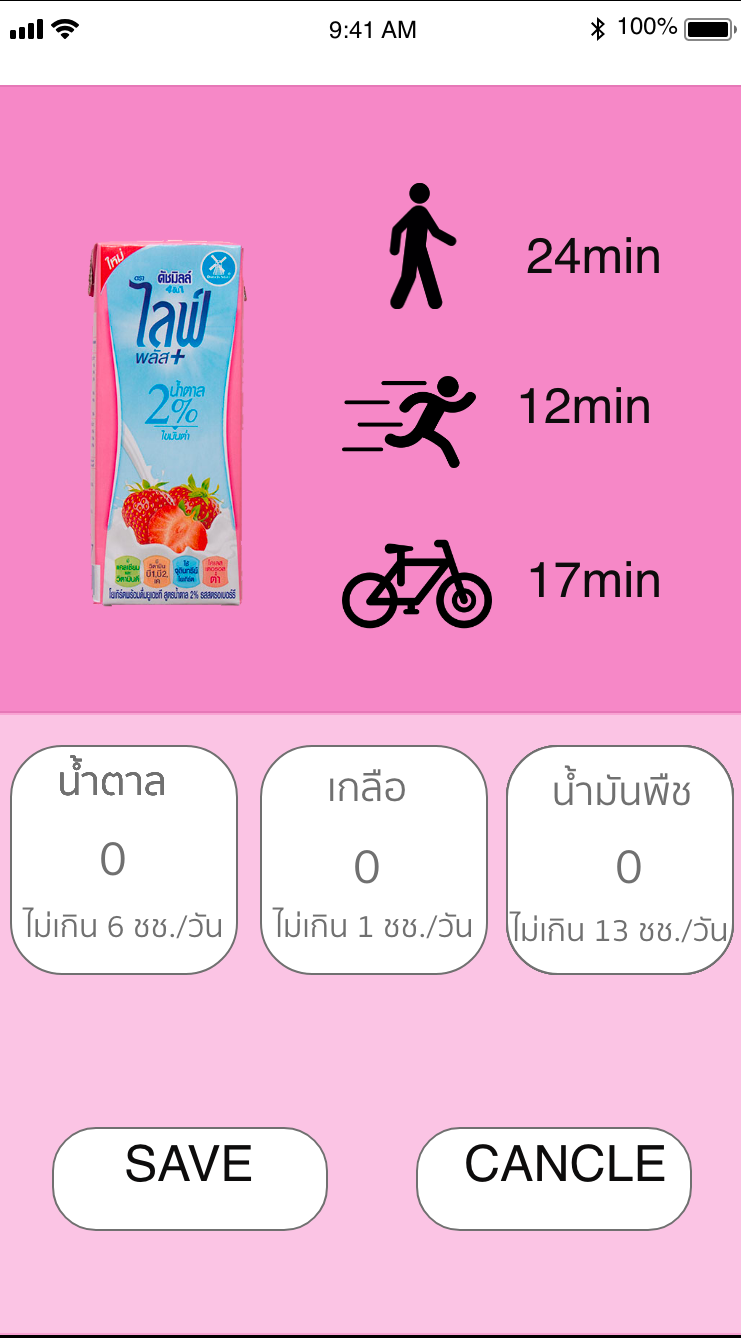
\includegraphics[width=0.2\textwidth]{Figures/3/UIDESIGN/6}
					\caption{หน้าจอ แสดงข้อมูลอาหาร}
					\label{Fig:6}
				\end{figure}
				จากภาพที่ \ref{Fig:6} หน้าจอแสดงข้อมูลอาหารจะแสดงขึ้นมาหลังจากที่ผู้ใช้ทำการกดที่ปุ่มสแกนอาหาร ในหน้าจอนี้หากผู้ใช้ทำการกดปุ่ม SAVE จะเป็นการบันทึกข้อมูลอาหารลงในระบบ


				\item การออกแบบหน้าจอแสดงอาหารที่เพิ่มโดยผู้ใช้
				\begin{figure}[H]
								\centering
								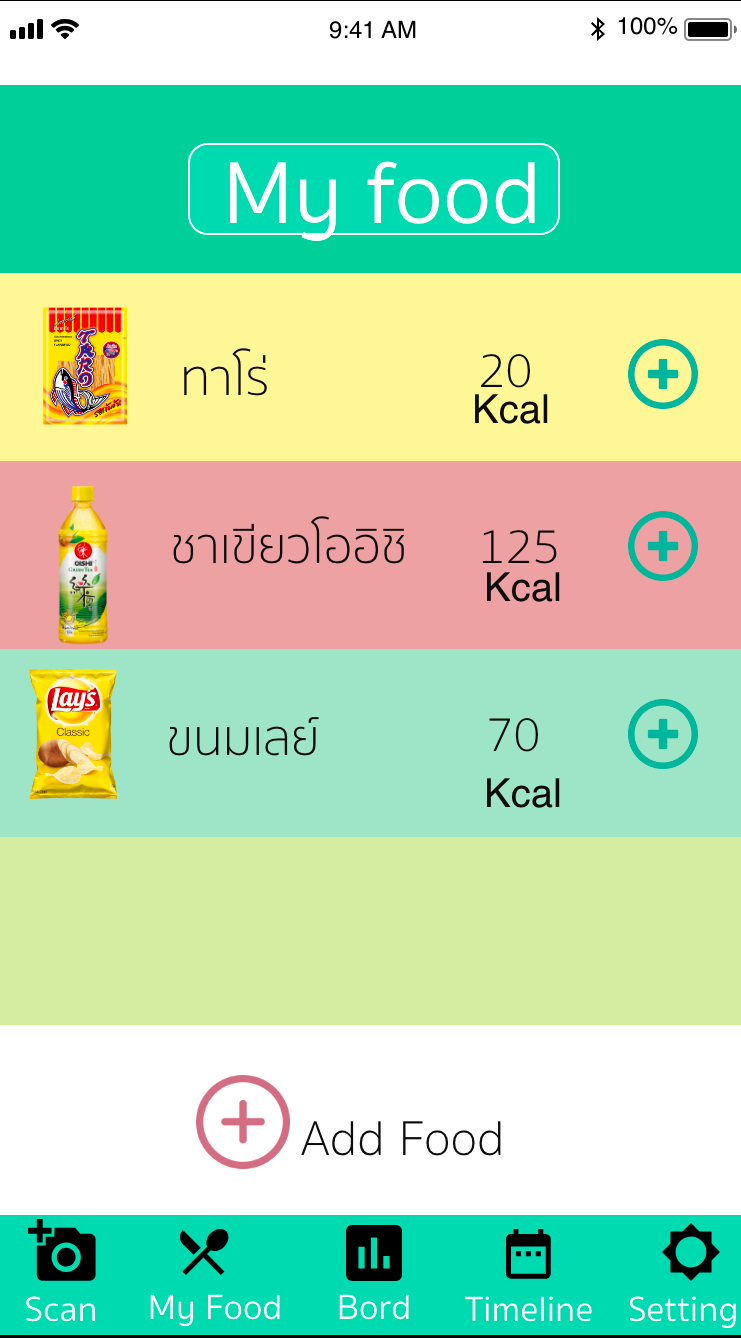
\includegraphics[width=0.2\textwidth]{Figures/3/UIDESIGN/7}
								\caption{หน้าจอ แสดงอาหารที่เพิ่มโดยผู้ใช้}
								\label{Fig:7}
							\end{figure}
							จากภาพที่ \ref{Fig:7} ในหน้าจอนี้จะแสดงอาหารที่ผู้ใช้เพิ่มเข้ามาด้วยผู้ใช้เอง หากกดที่ปุ่ม ADD Food จะทำการแสดงหน้าจอสำหรับเพิ่มอาหาร

			
							\item การออกแบบหน้าจอสำหรับเพิ่มอาหาร
							\begin{figure}[H]
											\centering
											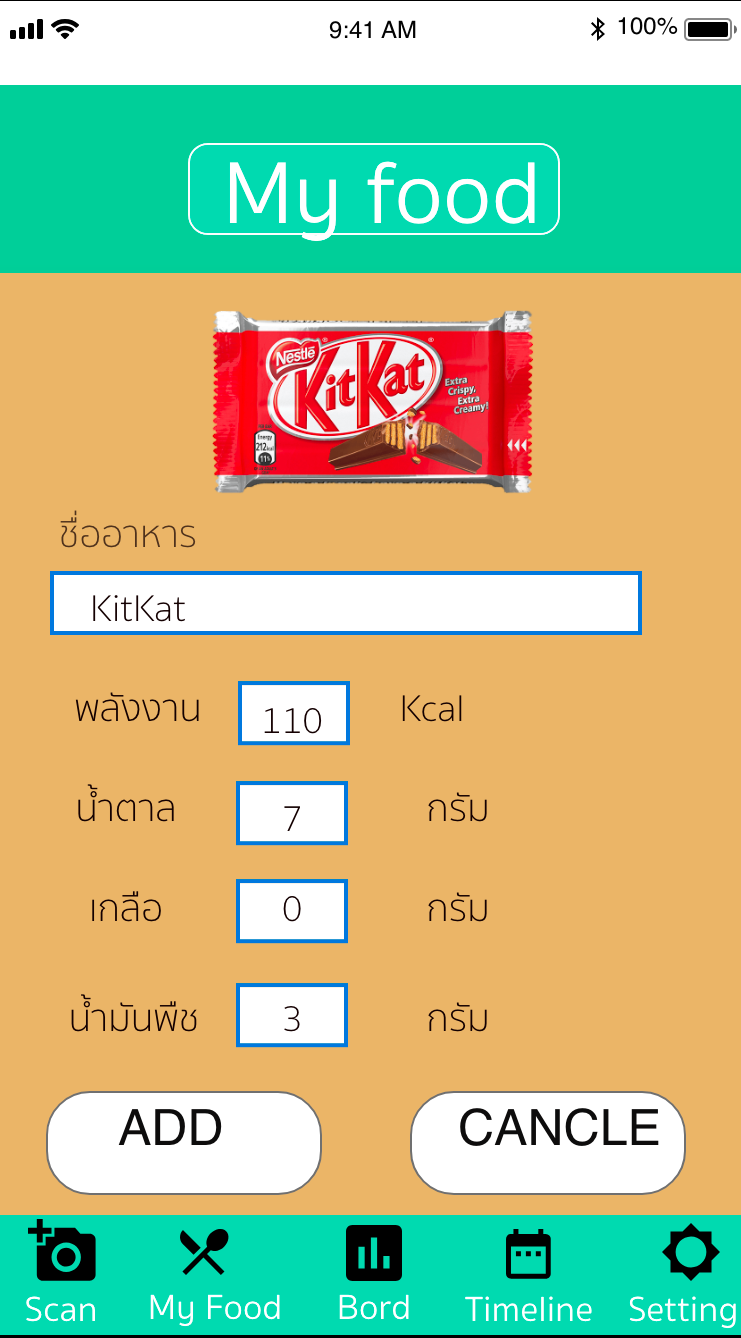
\includegraphics[width=0.2\textwidth]{Figures/3/UIDESIGN/8.png}
											\caption{หน้าจอ สำหรับเพิ่มอาหาร }
											\label{Fig:8.png}
										\end{figure}
										จากภาพที่ \ref{Fig:8.png} หน้าจอเพิ่มอาหารนี้จะมีช่องให้ใส่ชื่อและข้อมูลของอาหาร หากผู้ใช้ทำการกดปุ่ม ADD จะทำการเพิ่มอาหารเข้าไปในระบบ

							\item การออกแบบหน้าจอแก้ไขอาหาร
							\begin{figure}[H]
											\centering
											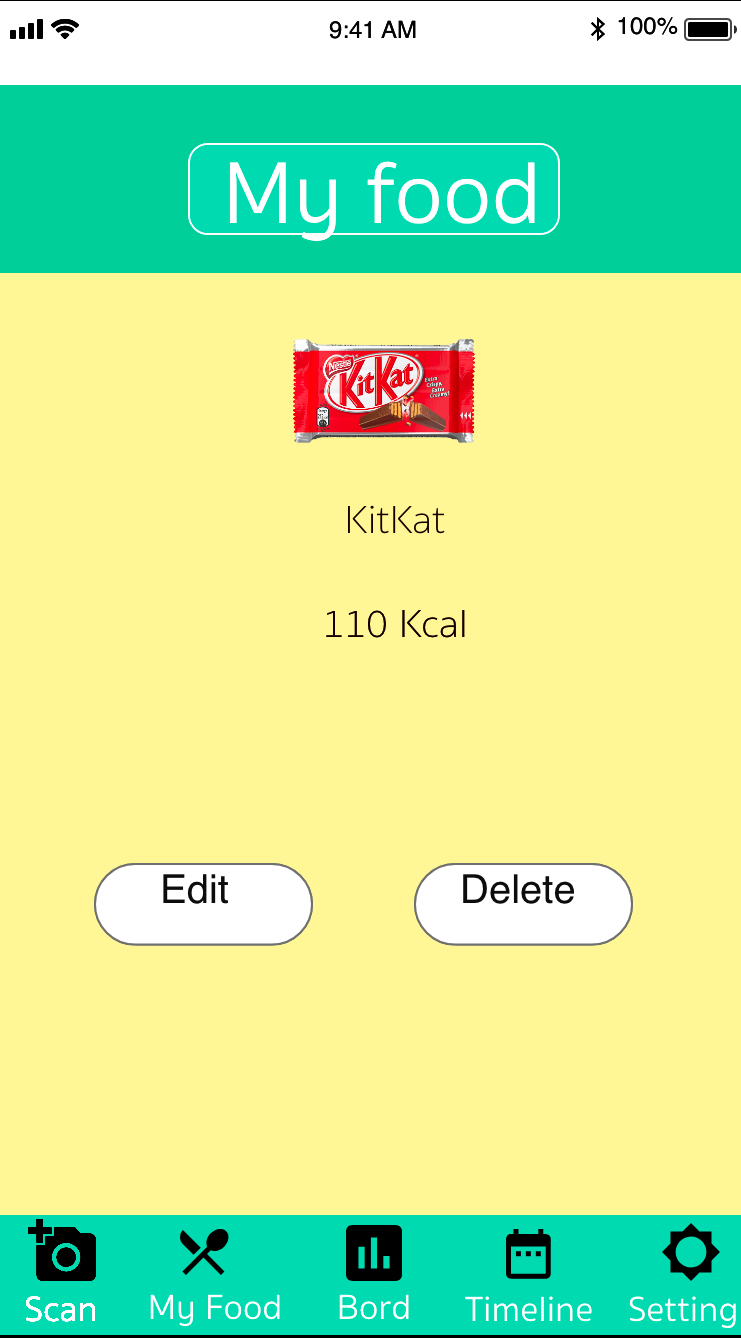
\includegraphics[width=0.2\textwidth]{Figures/3/UIDESIGN/9.png}
											\caption{หน้าจอ แก้ไขอาหาร }
											\label{Fig:9.png}
										\end{figure}
										จากภาพที่ \ref{Fig:9.png} หน้าจอแก้ไขอาหาร ผู้ใช้ต้องทำการกดที่ชื่ออาหาร หน้าจอแก้ไขอาหารจึงจะแสดงขึ้นมา ในหน้าจอแก้ไขอาหารผู้ใช้สามารถแก้ไขและลบข้อมูลอาหารได้


		\item การออกแบบหน้าจอจัดการข้อมูลผู้ใช้
							\begin{figure}[H]
											\centering
											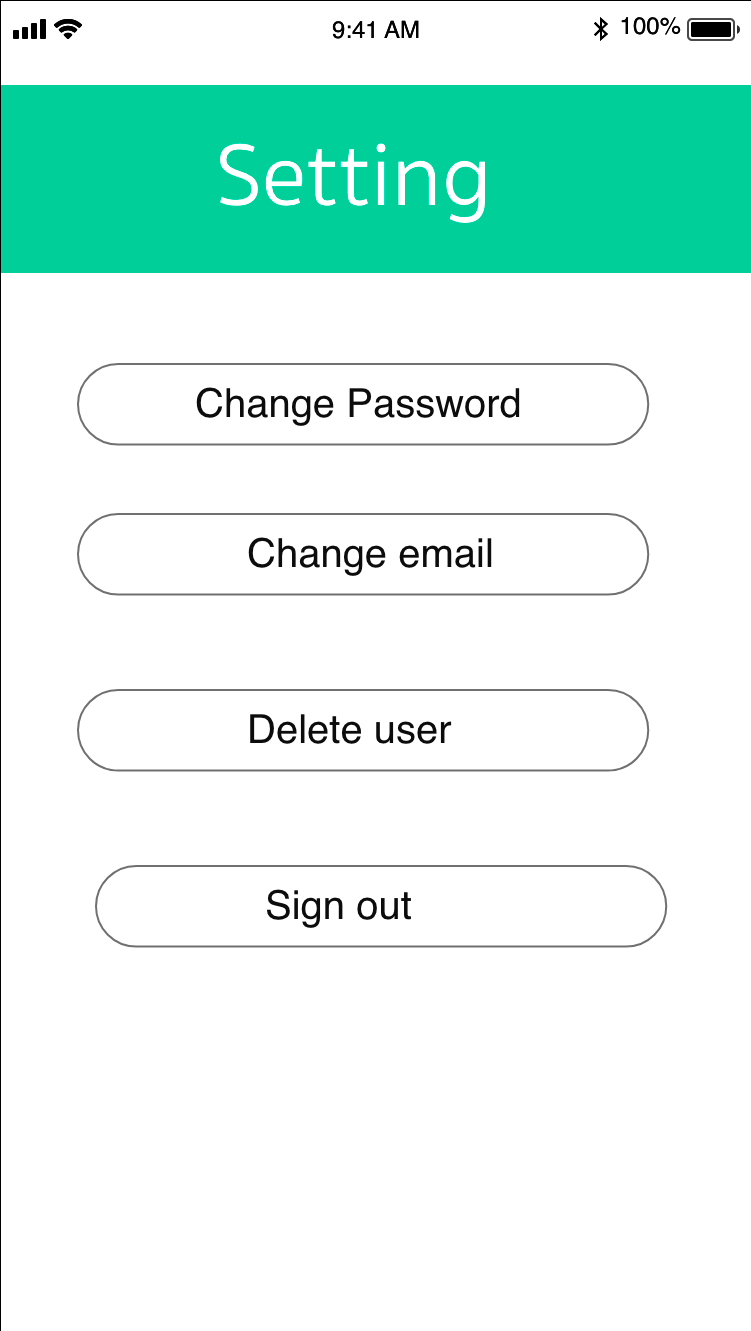
\includegraphics[width=0.2\textwidth]{Figures/3/UIDESIGN/3.png}
											\caption{หน้าจอ จัดการข้อมูลผู้ใช้ }
											\label{Fig:3.png}
										\end{figure}
										จากภาพที่ \ref{Fig:3.png} ในหน้าจัดการข้อมูลผู้ใช้ ผู้ใช้สามารถแก้ไขอีเมล รหัสผ่าน  และออกจากระบบ ได้ 

\section{Use Case Diagram}
	Use Case Diagram เป็นแผนผังเพื่อแสดงฟังก์ชันแสดงการทำงานของระบบโดยรวม แสดงส่วนประกอบในระบบและกิจกรรมที่เกิดขึ้นในระบบซึ่งในระบบระบบกองทุนเงินให้กู้ยืมเพื่อการศึกษา คณะวิทยาศาสตร์ มหาวิทยาลัยอุบลราชธานี ผู้ใช้จำเป็นต้องเข้าสู่ระบบเพื่อใช้งานระบบ สัญลักษณ์ที่ใช้ในการเขียน Use Case Diagram แสดงในตารางที่ \ref{tab:use-case2}
	\begin{table}[H]
		\caption{สัญลักษณ์ของ Use case Diagram}
		\label{tab:use-case2}
		\begin{tabular}{|c|p{10cm}|}
		\hline
		\textbf{สัญลักษณ์} & \multicolumn{1}{c|}{\textbf{การใช้งาน}} \\ \hline
		\raisebox{-\totalheight}{Use case}
		& \setstretch{1.5} {Use case คือส่วนย่อยของระบบงาน แทนด้วยวงรีและชื่อของ Use case ภายในวงรี} \\ \hline
		\raisebox{-\totalheight}{
\includegraphics[height=1.5cm]{Figures/table/use-case/2}}
		& \setstretch{1.5} {Actor คือบุคคลหรือระบบงานอื่นที่ใช้งานระบบหรือได้รับประโยชน์จากระบบซึ่งอยู่ภายนอกระบบ แทนด้วยรูปคนและมีชื่อบทบาทการใช้งานระบบ} \\ \hline
		\raisebox{-\totalheight}{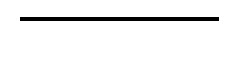
\includegraphics[width=3cm]{Figures/table/use-case/3}}
		& \setstretch{1.5} {เส้นตรงที่แสดงถึงการใช้งาน Use case ของผู้กระทำ} \\ \hline
		\raisebox{-\totalheight}{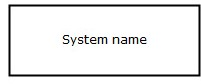
\includegraphics[width=0.3\textwidth]{Figures/table/use-case/4}}
		& \setstretch{1.5} {กรอบสี่เหลี่ยมแสดงถึงขอบเขตของระบบโดยแสดงชื่อระบบภายในหรือด้านบนกรอกสี่เหลี่ยม Use case อยู่ภายในกรอบสี่เหลี่ยม และ actor อยู่ภายนอกกรอบสี่เหลี่ยม} \\ \hline
		\raisebox{-\totalheight}{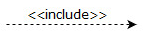
\includegraphics[width=0.3\textwidth]{Figures/table/use-case/5}}
		& \setstretch{1.5} {ความสัมพันธ์แบบ <<includes>> แสดงว่า Use case หนึ่งดำเนินการตามขั้นตอนของ Use case อื่น โดยแทนด้วยสัณลักษณ์ลูกศรเส้นประ ซึ่ง Use case ที่หางลูกศรเรียกใช้งาน Use case ที่หัวลูกศรทุกครั้งที่มีการทำงาน} \\ \hline
		\raisebox{-\totalheight}{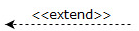
\includegraphics[width=0.3\textwidth]{Figures/table/use-case/6}}
		& \setstretch{1.5} {ความสัมพันธ์แบบ <<extend>> แสดงว่า Use case หนึ่งดำเนินการตามขั้นตอนของ Use case อื่น โดยแทนด้วยสัญลักษณ์ลูกศรเส้นประ ซึ่ง Use case ที่หัวลูกศรเรียกใช้งาน Use case ที่หางลูกศร แต่การใช้งานไม่จำเป็นต้องเกิดขึ้นทุกครั้งขึ้นอยู่กับเงื่อนไขระหว่างการทำงาน} \\ \hline
		\end{tabular}
	\end{table}

	\begin{figure}[H]
		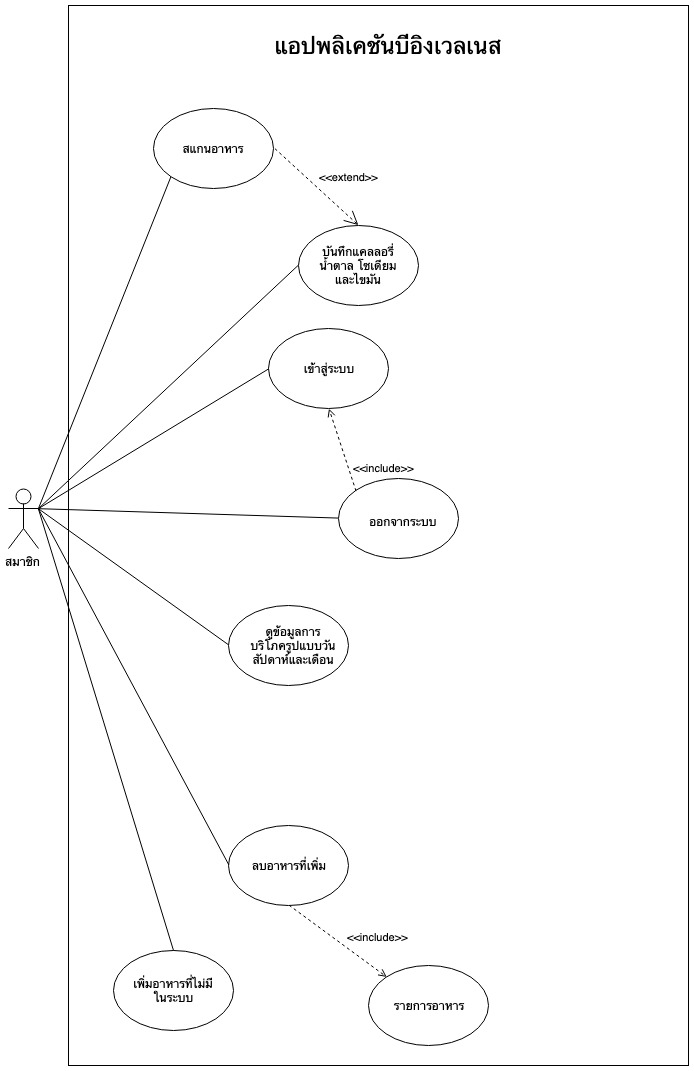
\includegraphics[width=0.9\textwidth]{Figures/3/usecase/usecase.jpg}
		\caption{Use Case Diagram ของแอปพลิเคชันบีอิงเวลเนส}
		\label{Fig:usecase}
	\end{figure}
	
	\begin{table}[H]
		\centering
		\caption{อธิบาย Use Case หน้าที่ของระบบ ในภาพที่ \ref{Fig:usecase}}
		\label{tab:usecase}
		\resizebox{\totalheight}{!}{\textwidth}{%
			\begin{tabular}{|c|p{8cm}|}
				\hline
				\multicolumn{1}{|c|}{\textbf{Use Case}} & \multicolumn{1}{c|}{\textbf{คำอธิบาย}} \\ \hline
				สแกนอาหาร & สมาชิกสามารถสแกนอาหารแต่ไม่จำเป็นต้องบันทึกข้อมูลการบริโภคทุกครั้ง \\ \hline
				บันทึกแคลลอรี่ น้ำตาล โซเดียมและไขมัน &  การบันทึกข้อมูลการบริโภคสมาชิกไม่จำต้องทำการสแกนทุกครั้ง \\ \hline
				เข้าสู่ระบบ & สมาชิกสามารถทำการเข้าสู่ระบบได้ \\ \hline
				ออกจากระบบ & สมาชิกจะต้องทำการเข้าสู่ระบบก่อนจึงจะสามารถออกจากระบบได้ \\ \hline
				ดูข้อมูลการบริโภครูปแบบวัน สัปดาห์และเดือน & หลังจากสมาชิกทำการเข้าสู่ระบบแล้วสมาชิกสามารถดูข้อมูลการบริโภคในรูปแบบวัน
				 สัปดาห์และเดือนได้  \\ \hline
				ลบอาหารที่เพิ่ม &  สมาชิกสามารถลบอาหารที่เพิ่มเข้ามาได้ด้วยการเลือกที่รายการอาหาร \\ \hline
				เพิ่มอาหารที่ไม่มีในระบบ &  สมาชิกสามารถเพิ่มอาหารที่ไม่มีในระบบเองได้   \\ \hline
			\end{tabular}%
		}
	\end{table}
	% Please add the following required packages to your document preamble:
	% \usepackage{graphicx}
	\begin{table}[H]
		\centering
		\caption{Use Case สแกนอาหาร}
		\label{tab:usecase}
		\resizebox{\totalheight}{!}{\textwidth}{%
			\begin{tabular}{|p{10cm}|p{10cm}|}
				\hline
				\multicolumn{1}{|c|}{\textbf{Use Case Title : สแกนอาหาร}} & \multicolumn{1}{c|}{\textbf{Use case Id : 1 }} \\ \hline
				\multicolumn{2}{|p{\linewidth}|}{Primary Actor : สมาชิก} \\ \hline
			    \multicolumn{2}{|p{\linewidth}|}{Main Flow : สมาชิกจะต้องทำการเข้าสู่ระบบก่อนจึงจะสามารถทำการสแกนได้} \\ \hline
			    \multicolumn{2}{|p{\linewidth}|}{Exceptional Flow ที่ 1 : หากผู้ใช้ไม่เชื่อมต่ออินเทอร์เน็ต จะไม่สามารถทำการสแกนได้} \\ \hline
			\end{tabular}%
		}
	\end{table}
	\begin{table}[H]
		\centering
		\caption{Use Case บันทึกแคลลอรี่ น้ําตาล โซเดียมและไขมัน}
		\label{tab:usecase}
		\resizebox{\totalheight}{!}{\columnwidth}{%
			\begin{tabular}{|p{7cm}|p{7cm}|}
				\hline
				\multicolumn{1}{|c|}{\textbf{Use Case Title : บันทึกแคลลอรี่ น้ําตาล โซเดียมและไขมัน}} & \textbf{Use case Id : 2 } \\ \hline
				\multicolumn{2}{|l|}{Primary Actor : สมาชิก} \\ \hline
				\multicolumn{2}{|p{\linewidth}|}{Main Flow : หากสมาชิกต้องการบันทึกสมาชิกสามารทำการสแกนหรือบันทึกจากอาหารที่เพิ่มเองได้  } \\ \hline
				\multicolumn{2}{|p{\linewidth}|}{Exceptional Flow ที่ 1 : หากสมาชิกไม่เชื่อมต่ออินเทอร์เน็ต จะไม่สามารถทำการบันทึกข้อมูลอาหารได้} \\ \hline
			\end{tabular}%
		}
	\end{table}

	\begin{table}[H]
		\centering
		\caption{Use Case เข้าสู่ระบบ}
		\label{tab:usecase}
		\resizebox{\totalheight}{!}{\textwidth}{%
			\begin{tabular}{|p{7cm}|p{7cm}|}
				\hline
				\multicolumn{1}{|c|}{\textbf{Use Case Title : ดาวน์โหลดเอกสาร}} & \textbf{Use case Id : 3 } \\ \hline
				\multicolumn{2}{|l|}{Primary Actor : สมาชิก} \\ \hline
				\multicolumn{2}{|p{\linewidth}|}{Main Flow : สมาชิกต้องทำการสมัครสมาชิกก่อนจึงจะสามารถทำการเข้าสู่ระบบได้				} \\ \hline
				\multicolumn{2}{|p{\linewidth}|}{Exceptional Flow ที่ 1 : หากสมาชิกไม่เชื่อมต่ออินเทอร์เน็ต จะไม่สามารถทำการเข้าสู่ระบบได้} \\ \hline
				\multicolumn{2}{|p{\linewidth}|}{Exceptional Flow ที่ 2 : หากสมาชิกไม่ทำการสมัครสมาชิกจะไม่สามารถทำการเข้าสู่ระบบได้ } \\ \hline
			\end{tabular}%
		}
		\end{table}
		
		\begin{table}[H]
			\centering
			\caption{Use Case ออกจากระบบ}
			\label{tab:usecase}
			\resizebox{\totalheight}{!}{\textwidth}{%
				\begin{tabular}{|p{10cm}|p{10cm}|}
					\hline
					\multicolumn{1}{|c|}{\textbf{Use Case Title : ออกจากระบบ}} & \multicolumn{1}{c|}{\textbf{Use case Id : 4 }} \\ \hline
					\multicolumn{2}{|l|}{Primary Actor : สมาชิก} \\ \hline
					\multicolumn{2}{|p{\linewidth}|}{Main Flow : สมาชิกจะต้องทำการเข้าสู่ระบบก่อนจึงจะสามารถออกจากระบบได้ } \\ \hline
					\multicolumn{2}{|p{\linewidth}|}{Exceptional Flow ที่ 1 : หากผู้ใช้ไม่ทำการเข้าสู่ระบบ จะไม่สามารถออกจากระบบได้ } \\ \hline
				\end{tabular}%
			}
		\end{table}
		
		\begin{table}[H]
			\centering
			\caption{Use Case ดูข้อมูลการบริโภครูปแบบวัน สัปดาห์และเดือน}
			\label{tab:usecase}
			\resizebox{\totalheight}{!}{\textwidth}{%
				\begin{tabular}{|c|p{10cm}|}
					\hline
					\multicolumn{1}{|c|}{\textbf{Use Case Title : ดูข้อมูลการบริโภครูปแบบวัน สัปดาห์และเดือน}} & \multicolumn{1}{c|}{\textbf{Use case Id : 5 }} \\ \hline
					\multicolumn{2}{|l|}{Primary Actor : สมาชิก} \\ \hline
					\multicolumn{2}{|p{\linewidth}|}{Main Flow : เมื่อสมาชิกทำการเข้าสู่ระบบแล้ว สมาชิกสามารถดูข้อมูลการบริโภคในรูปแบบวัน สัปดาห์และเดือนได้ } \\ \hline
					\multicolumn{2}{|p{\linewidth}|}{Exceptional Flow ที่ 1 : หากผู้ใช้ไม่เชื่อมต่ออินเทอร์เน็ต จะไม่สามารถดูข้อมูลการบริโภคในรูปแบบวัน สัปดาห์และเดือนได้} \\ \hline
				\end{tabular}%
			}
		\end{table}
	
		\begin{table}[H]
			\centering
			\caption{Use Case ลบอาหารที่เพิ่ม}
			\label{tab:usecase}
			\resizebox{\totalheight}{!}{\textwidth}{%
				\begin{tabular}{|c|p{10cm}|}
					\hline
					\multicolumn{1}{|c|}{\textbf{Use Case Title : ลบอาหารที่เพิ่ม}} & \multicolumn{1}{c|}{\textbf{Use case Id : 6 }} \\ \hline
					\multicolumn{2}{|l|}{Primary Actor : สมาชิก} \\ \hline
					\multicolumn{2}{|p{\linewidth}|}{Main Flow :  สมาชิกสามารถทำการลบอาหารได้ด้วยการเลือกที่เมนูอาหาร} \\ \hline
					\multicolumn{2}{|p{\linewidth}|}{Exceptional Flow ที่ 1 : หากสมาชิกไม่เชื่อมต่ออินเทอร์เน็ต จะไม่สามารถทำการลบอาหารได้} \\ \hline
				\end{tabular}%
			}
		\end{table}	
		
		\begin{table}[H]
			\centering
			\caption{Use Case เพิ่มอาหารท่ีไม่มีในระบบ}
			\label{tab:usecase}
			\resizebox{\totalheight}{!}{\textwidth}{%
				\begin{tabular}{|c|p{10cm}|}
					\hline
					\multicolumn{1}{|c|}{\textbf{Use Case Title : เพิ่มอาหารท่ีไม่มีในระบบ}} & \multicolumn{1}{c|}{\textbf{Use case Id : 7 }} \\ \hline
					\multicolumn{2}{|l|}{Primary Actor : สมาชิก} \\ \hline
					\multicolumn{2}{|p{\linewidth}|}{Main Flow :  สมาชิกสามารถเพิ่มอาหารที่ไม่มีในระบบได้ด้วยการกดปุ่ม ADD  } \\ \hline
					\multicolumn{2}{|p{\linewidth}|}{Exceptional Flow ที่ 1 : หากสมาชิกไม่เชื่อมต่ออินเทอร์เน็ต จะไม่สามารถเพิ่มอาหารได้} \\ \hline
				\end{tabular}%
			}
		\end{table}	
%		\begin{table}[H]
%			\centering
%			\caption{Use Case สมัครสมาชิก}
%			\label{tab:usecase}
%			\resizebox{\totalheight}{!}{\textwidth}{%
%				\begin{tabular}{|c|p{10cm}|}
%					\hline
%					\multicolumn{1}{|c|}{\textbf{Use Case Title : สมัครสมาชิก}} & \multicolumn{1}{c|}{\textbf{Use case Id : 8 }} \\ \hline
%					\multicolumn{2}{|l|}{Primary Actor : นักศึกษา} \\ \hline
%					\multicolumn{2}{|l|}{Stakeholder Actor : -} \\ \hline
%					\multicolumn{2}{|p{\linewidth}|}{Main Flow : เมื่อนักศึกษาต้องการใช้งานระบบทั้งหมดของกองทุนจำเป็นต้องเข้าสู่ระบบก่อน หากยังไม่มีบัญชีสามารถสมัครได้โดยต้องกรอกข้อมูลอีเมลและรหัสผ่าน} \\ \hline
%					\multicolumn{2}{|p{\linewidth}|}{Exceptional Flow ที่ 1 : หากผู้ใช้ไม่เชื่อมต่ออินเทอร์เน็ต จะไม่สามารถสมัครสมาชิกได้} \\ \hline
%				\end{tabular}%
%			}
%		\end{table}	
%		 \begin{table}[H]
%		 	\centering
%		 	\caption{Use Case เข้าสู่ระบบ}
%		 	\label{tab:usecase}
%		 	\resizebox{\totalheight}{!}{\textwidth}{%
%		 		\begin{tabular}{|c|p{10cm}|}
%		 			\hline
%		 			\multicolumn{1}{|c|}{\textbf{Use Case Title : เข้าสู่ระบบ}} & \multicolumn{1}{c|}{\textbf{Use case Id : 9 }} \\ \hline
%		 			\multicolumn{2}{|l|}{Primary Actor : นักศึกษา} \\ \hline
%		 			\multicolumn{2}{|l|}{Stakeholder Actor : -} \\ \hline
%		 			\multicolumn{2}{|p{\linewidth}|}{Main Flow : เมื่อนักศึกษาต้องการใช้งานระบบทั้งหมดของกองทุนจำเป็นต้องเข้าสู่ระบบก่อนโดยต้องกรอกข้อมูลอีเมลและรหัสผ่าน} \\ \hline
%		 			\multicolumn{2}{|p{\linewidth}|}{Exceptional Flow ที่ 1 : หากผู้ใช้ไม่เชื่อมต่ออินเทอร์เน็ต จะไม่สามารถเข้าสู่ระบบได้} \\ \hline
%		 		\end{tabular}%
%		 	}
%		 \end{table}	
	
\newpage

\section{Class Diagram}
	Class Diagram คือแผนภาพที่ใช้แสดงคลาสและความสัมพันธ์ในแบบต่างๆ ระหว่างคลาส สัญลักษณ์ที่ใช้ในการเขียน Class Diagram แสดงในตารางที่ \ref{tab:class2} 
	\begin{center}
	\begin{table}[H]
		\centering
		\caption{สัญลักษณ์ของ Class Diagram}
		\label{tab:class2}
		\begin{tabular}{|c|p{10cm}|}
			\hline
			\textbf{สัญลักษณ์} & \multicolumn{1}{c|}{\textbf{การใช้งาน}} \\ \hline
			\raisebox{-\totalheight}{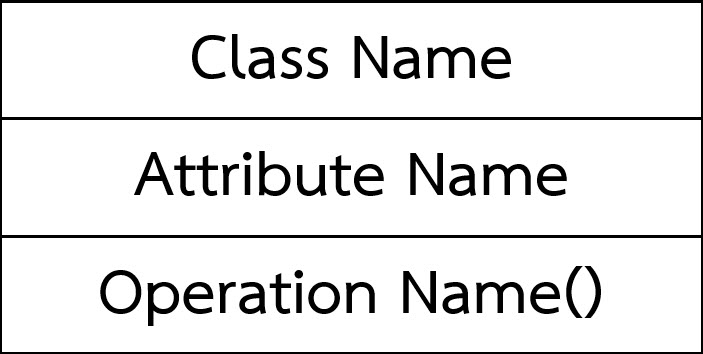
\includegraphics[width=0.3\textwidth]{Figures/table/class/11}}
			& \setstretch{1.5} {คลาส สัญลักษณ์แทนด้วยสี่เหลี่ยมแบ่งเป็น 3 ส่วน 
				ส่วนบน เป็นชื่อของ class ส่วนกลาง เป็นชื่อ Attribute และส่วนล่างเป็น Operation Name หรือ Method ใช้สำหรับเขียนฟังก์ชันในการทำงานของคลาสนั้น ๆ
				ชนิดของ Visibility ของ Method และ Attribute
				แบ่งเป็น 3 ชนิด ได้แก่
				\begin{enumerate}
					\item Public แทนสัญลักษณ์ด้วยเครื่องหมายบวก (+)
					\item Private แทนสัญลักษณ์ด้วยเครื่องหมายลบ (-)
					\item Protected แทนสัญลักษณ์ด้วยเครื่องหมายชาร์ป (#)
				\end{enumerate}
			} \\ \hline
			\raisebox{-\totalheight}{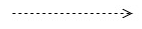
\includegraphics[width=0.3\textwidth]{Figures/table/class/1}}
			& \setstretch{1.5} {Dependency Relationship หมายความว่า คลาสที่อยู่ฝั่งต้นลูกศรสามารถเรียกใช้คลาสที่อยู่ฝั่งหัวลูกศร}
			\\ \hline
			\raisebox{-\totalheight}{
\includegraphics[width=0.35\textwidth]{Figures/3/Class/aggre}}
			& \setstretch{1.5} {Composition Relationship เป็นความสัมพันธ์ระหว่างออบเจ็กต์หรือคลาสแบบขึ้นต่อกันและมีความเกี่ยวข้องกันเสมอ} \\ \hline
			\raisebox{-\totalheight}{
\includegraphics[width=0.3\textwidth]{Figures/3/Class/implement}}
			& \setstretch{1.5} {Realization Relationship เป็นความสัมพันธ์ระหว่าง Object หรือ Class ในลักษณะของการสืบทอดคุณสมบัติจาก Class หนึ่ง (Super class) ไปยังอีก Class หนึ่ง (Subclass)} \\ \hline
			\raisebox{-\totalheight}{
\includegraphics[width=50,height=50]{Figures/table/class/connector}}
			& \setstretch{1.5} {Connector เป็นสัญลักษณ์แทนด้วยรูปห้าเหลี่ยมและมีชื่ออยู่ตรงกลาง จะสร้างสัญลักษณ์นี้ไว้เมื่อต้องการเชื่อมต่อคลาสที่อยู่คนละหน้า} \\ \hline
		\end{tabular}
	\end{table}
	\end{center}

\newpage
	%IMAGE of class

	Class Diagram แสดงความสัมพันธ์ในรูปแบบต่างๆ ระหว่างคลาสของแอปพลิเคชันระบบกองทุนเงินให้กู้ยืมเพื่อการศึกษา คณะวิทยาศาสตร์ มหาวิทยาลัยอุบลราชธานี อธิบายได้ตามภาพที่ \ref{Fig:MainActivity20C} ดังต่อไปนี้
	

	\begin{figure}[H]

		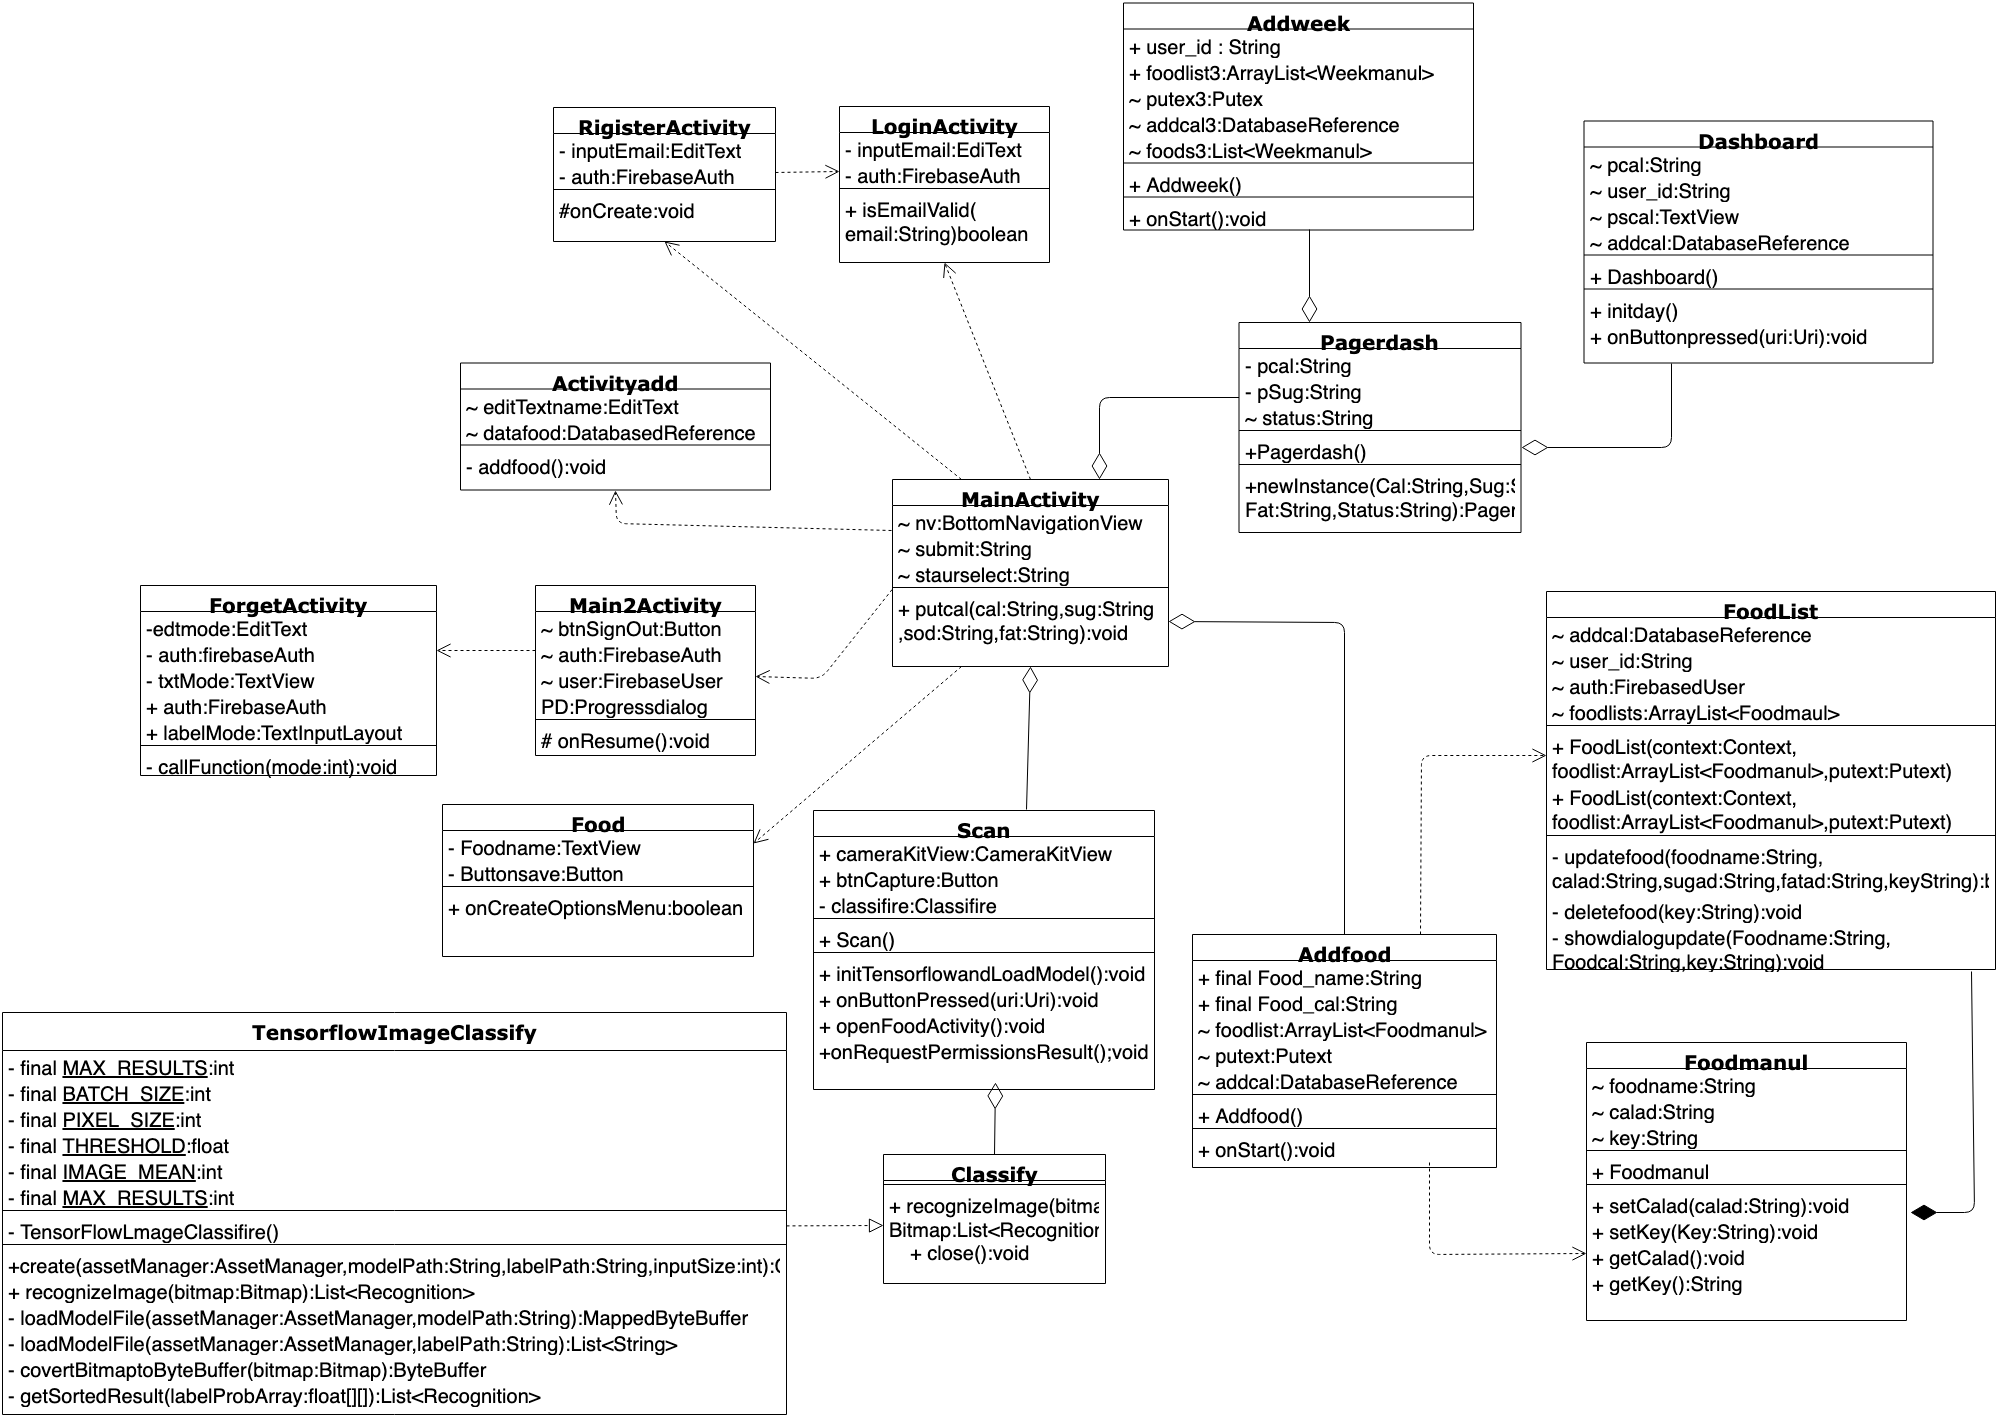
\includegraphics[width=1.1\columnwidth]{Figures/3/Class/class14.png}
		\caption{Class Diagram ของแอปพลิเคชันบีอิงเวลเนส}
		\label{Fig:MainActivity20C}
	\end{figure}


	% TABLE of class
\newpage	
	จากรูปภาพที่ \ref{Fig:MainActivity20C} สามารถอธิบายแผนภาพ Class Diagram ได้ดังนี้
	\begin{table}[H]
		\centering
		\caption{อธิบาย Class Diagram ของแอปพลิเคชันบีอิงเวลเนส}
		\label{tab:class}
		\begin{tabular}{|c|p{10cm}|}
			\hline
			\textbf{Class Diagram} & \multicolumn{1}{c|}{\textbf{คำอธิบาย}} \\ \hline
			\raisebox{-\totalheight}{LoginActivity}
			& \setstretch{1.5} {คลาส LoginActivity จะถูกเรียกใช้เมื่อสมาชิกเปิดแอพพลิเคชัน โดยวัตถุประสงค์การทำงานของคลาสนี้คือ เพื่อให้สมาชิกทำการเข้าสู่ระบบและสมัครสมาชิก } \\ \hline
			\raisebox{-\totalheight}{RigisterActivity}
			& \setstretch{1.5} {คลาส RigisterActivity จะถูกใช้งานเมื่อผู้ใช้กดปุ่ม SiGN UP โดยวัตถุประสงค์การทำงานของคลาสคือ เพื่อให้สมาชิกทำการสมัครสมาชิก} \\ \hline
			\raisebox{-\totalheight}{MainActivity}
			& \setstretch{1.5} {คลาส MainActivity เป็นคลาสหลักที่ใช้ในการทำงานของแอปพลิเคชันโดยการทำงานของคลาสนี้เน้นไปที่การเรียกใช้ Fragment โดยองค์ประกอบของคลาสนี้ประกอบไปด้วยคลาสของ Fragment ได้แก่ Pagerdash Myfood Scan} \\ \hline
			\raisebox{-\totalheight}{Main2Activiy}
			& \setstretch{1.5} {คลาส Main2Activiy เป็นคลาสที่ให้สมาชิกได้เลือกการจัดการบัญชีสมาชิก ได้แก่ เปลี่ยนอีเมล เปลี่ยนรหัสผ่าน ลบผู้ใช้ และออกจากระบบ} \\ \hline
			\raisebox{-\totalheight}{ForgetActivity}
			& \setstretch{1.5} {คลาส ForgetActivity  เป็นคลาสที่ทำการจัดการบัญชีสมาชิก ได้แก่ เปลี่ยนอีเมล เปลี่ยนรหัสผ่าน ลบผู้ใช้  } \\ \hline
			\raisebox{-\totalheight}{Activityadd}
			& \setstretch{1.5} {คลาส Activityadd  เป็นคลาสที่มีไว้สำหรับให้สมาชิกเพิ่มอาหารที่ไม่มีในระบบ } \\ \hline
			\raisebox{-\totalheight}{Food}
			& \setstretch{1.5} {คลาส Food  จะถูกใช้งานเมื่อสมาชิกทำการสแกนอาหาร โดยวัตถุประสงค์การทำงานของคลาสคือเพื่อแสดงข้อมูลอาหารที่สแกนได้ } \\ \hline

	\end{tabular}
\end{table}

\newpage
\begin{table}[H]
	\centering
	\caption{อธิบาย Class Diagram ของแอปพลิเคชันบีอิงเวลเนส(ต่อ)}
	\label{tab:class}
	\begin{tabular}{|c|p{10cm}|}
		\hline
		\textbf{Class Diagram} & \multicolumn{1}{c|}{\textbf{คำอธิบาย}} \\ \hline
		\raisebox{-\totalheight}{Pagerdash}
		& \setstretch{1.5} {คลาส Pagerdash เป็นคลาสหลักที่ใช้ในการจัดการ Tab เมนูในการเลื่อนเพื่อดูรูปแบบของข้อมูลการบริโภค} \\ \hline
		\raisebox{-\totalheight}{Addweek}
		& \setstretch{1.5} {คลาส Addweek  เป็นคลาสที่จะแสดงเมื่อสมาชิกทำการเลื่อนมาที่ Tab Week เป็นคลาสที่แสดงข้อมูลการบริโภคในรูปแบบสัปดาห์} \\ \hline
		\raisebox{-\totalheight}{Dashboard}
		& \setstretch{1.5} {คลาส Dashboard เป็นคลาสหลักที่จะถูกเรียกใช้เมื่อผู้ใช้ทำการเปิดแอปพลิเคชันหลังจากทำการเข้าสู่ระบบแล้ว โดยวัตถุประสงค์การทำงานของคลาสนี้คือ แสดงข้อมูลการบริโภคในรูปแบบวัน} \\ \hline
		\raisebox{-\totalheight}{Addfood}
		& \setstretch{1.5} {คลาส Addfood เป็นคลาสที่จะแสดงเมื่อผู้ใช้เลือกเมนู My food โดยวัตถุประสงค์การทำงานของคลาสคือแสดงรายการอาหารที่เพิ่มเข้ามา} \\ \hline
		\raisebox{-\totalheight}{FoodList}
		& \setstretch{1.5} {คลาส FoodList เป็นคลาสที่จะถูกใช้งานเมื่อคลาส Addfood ถูกใช้ โดยวัตถุประสงค์การทำงานของคลาสคือ จัดรูปแบบการแสดงรายการอาหาร} \\ \hline
		\raisebox{-\totalheight}{Foodmanul}
		& \setstretch{1.5} {คลาส Foodmanul เป็นคลาสที่กำหนดค่าต่างๆที่จำเป็นในการสร้างรายการอาหาร} \\ \hline
		\raisebox{-\totalheight}{Scan}
		& \setstretch{1.5} {คลาส Scan เป็นคลาสที่จะแสดงเมื่อผู้ใช้เลือกเมนู Scan โดยวัตถุประสงค์การทำงานของคลาสคือสแกนอาหาร} \\ \hline
		\raisebox{-\totalheight}{Classify}
		& \setstretch{1.5} {คลาส Classify เป็นคลาสที่ทำงานหลังจากสมาชิกทำการสแกน โดยวัตถุประสงค์การทำงานของคลาสคือแยกประเภทรูปภาพที่สมาชิกทำการถ่าย} \\ \hline
		\raisebox{-\totalheight}{TensorflowImageClassify}
		& \setstretch{1.5} {คลาส TensorflowImageClassify เป็นคลาสที่ทำงานร่วมกับคลาส  Classify โดยจะทำหน้าที่นำโมเดลเข้ามาเพื่อใช้ในการระบุภาพอาหารที่สมาชิกทำการถ่าย } \\ \hline
	\end{tabular}
\end{table}

\newpage
\section{Sequence Diagram}
	Sequence Diagram เป็น Diagram ที่แสดงขั้นตอนการทำงานของแต่ละ Use Case ระหว่าง Object ต่างๆ  โดย Sequence Diagram จะช่วยให้มองเห็นการทำงานของภาพรวมของระบบ ส่วนประกอบสัญลักษณ์ที่ใช้ในการเขียน Sequence Diagram 
	แสดงดังตารางที่ \ref{tab:Sequences}
	
	\begin{table}[H]
		\centering
		\caption{สัญลักษณ์ของ Sequence Diagram}
		\label{tab:Sequences}
		\begin{tabular}{| c	| p{10cm} |}
		\hline
		\textbf{สัญลักษณ์} & \multicolumn{1}{c|}{\textbf{การใช้งาน}} \\ \hline
		\raisebox{-\totalheight}{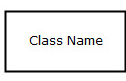
\includegraphics[width=0.17\textwidth]{Figures/table/Sequence/Sequence1}}
		& \setstretch{1.5} {Class แสดงถึงการทำงานของ Use Case ในการส่งหรือรับข้อความ แทนด้วยสัญลักษณ์สี่เหลี่ยมมีชื่อคลาสอยู่ภายใน} \\ \hline
		\raisebox{-\totalheight}{
\includegraphics[height=0.08\textheight]{Figures/table/Sequence/Sequence2}}
		& \setstretch{1.5} {Lifeline หรือเส้นอายุขัย แสดงช่วงเวลาตั้งแต่เริ่มสร้าง object ในคลาสนั้น จนกระทั่ง object นั้นถูกทำลาย สัญลักษณ์แทนด้วยเส้นประ} \\ \hline
		\raisebox{-\totalheight}{
\includegraphics[height=0.08\textheight]{Figures/table/Sequence/Sequence3}}
		& \setstretch{1.5} {Focus of control หรือจุดควบคุม เป็นจุดควบคุมที่ object ใช้ทำการส่งหรือรับข้อความ สัญลักษณ์แทนด้วยสี่เหลี่ยม} \\ \hline
		\raisebox{-\totalheight}{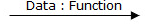
\includegraphics[width=0.3\textwidth]{Figures/table/Sequence/Sequence4}}
		& \setstretch{1.5} {Message คือ ข้อความที่รับส่งระหว่าง Object สัญลักษณ์แทนด้วยลูกศรและประกอบด้วย 2 ส่วน คือ ข้อมูล (Data) และฟังก์ชัน (Function)} \\ \hline
		\raisebox{-\totalheight}{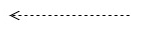
\includegraphics[width=0.3\textwidth]{Figures/table/Sequence/Sequence5}}
		& \setstretch{1.5} {Return Message เป็นข้อมูลที่ส่งกลับหลังจากทำงานเสร็จ} \\ \hline
		\raisebox{-\totalheight}{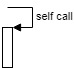
\includegraphics[height=0.08\textheight]{Figures/3/selfcall}}
		& \setstretch{1.5} {Self call เป็นการเรียกฟังชันก์การทำงานภายในตัวเอง} \\ \hline
		\raisebox{-\totalheight}{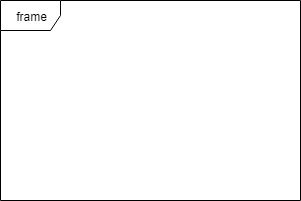
\includegraphics[height=0.1\textheight,width=0.3\textwidth]{Figures/3/frame}}
		& \setstretch{1.5} {สร้างกรอบการทำงานของโปรแกรม เพื่อให้รู้ขอบเขตของการทำงานเช่น ลูป(loop)} \\ \hline
		\end{tabular}
	\end{table}
%
%	Sequence Diagram ที่ใช้อธิบายการทำงานของระบบกองทุนเงินให้กู้ยืมเพื่อการศึกษา คณะวิทยสศาสตร์ มหาวิทยาลัยอุบลราชธานี มีรายละเอียดดังต่อไปนี้

\newpage
	\begin{landscape}
	\begin{figure}[H]
		\centering
		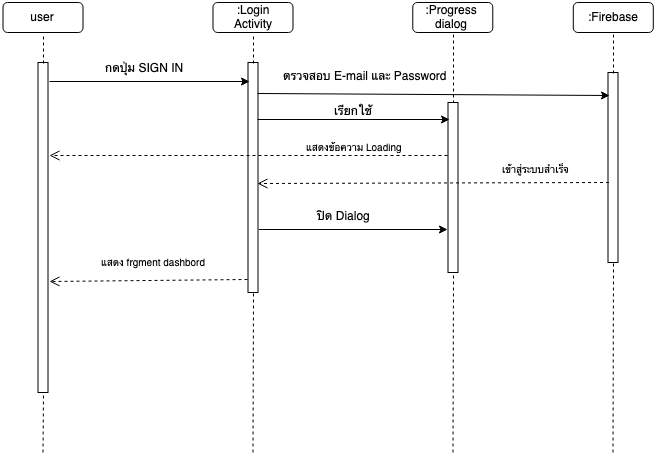
\includegraphics[width=0.95\columnwidth]
		{Figures/3/Sequence/sqlogin.png}
		\caption{Sequence Diagram การแสดงข่าวสาร}
		\label{Fig:Sequence-feed}
	\end{figure}
  \end{landscape}

	จากภาพที่ \ref{Fig:Sequence-feed} สามารถอธิบายแผนภาพ Sequence Diagram แสดงข่าวสาร ได้ดังนี้ เมื่อ
	ผู้ใช้เปิดโปรแกรมระบบจะเรียกใช้เมธอด onCreate() ที่คลาส MainActivity ระบบจะทำการสร้าง
	Fragment ขึ้นมาโดยใช้เมธอด onCreate() ที่คลาส FeedFragment เมื่อ FeedFragment ถูกติดตั้งบน MainActivity เมธอด callData() จะสืบค้นข้อมูลจากฐานข้อมูลบน Firebase FireStore และส่งข้อมูลที่ได้ไปแปลงที่คลาส FeedItemAdapter โดยมีการคืนค่าเป็นข้อมูลข่าวสารแต่ละแถวและในขั้นตอนสุดท้ายคลาส FeedFragment จะทำการแสดงรายการข้อมูลข่าวสารทั้งหมดออกทางหน้าจอ หากผู้ใช้มีการกดเลือกข่าวสารบางแถวคลาส FeedFragment จะทำการเรียกใช้ PostDetailActivity เพื่อแสดงรายละเอียดข้อมูลข่าวสารของแถวที่ถูกเลือก
	\begin{sidewaysfigure}
	\begin{figure}[H]
		\centering
		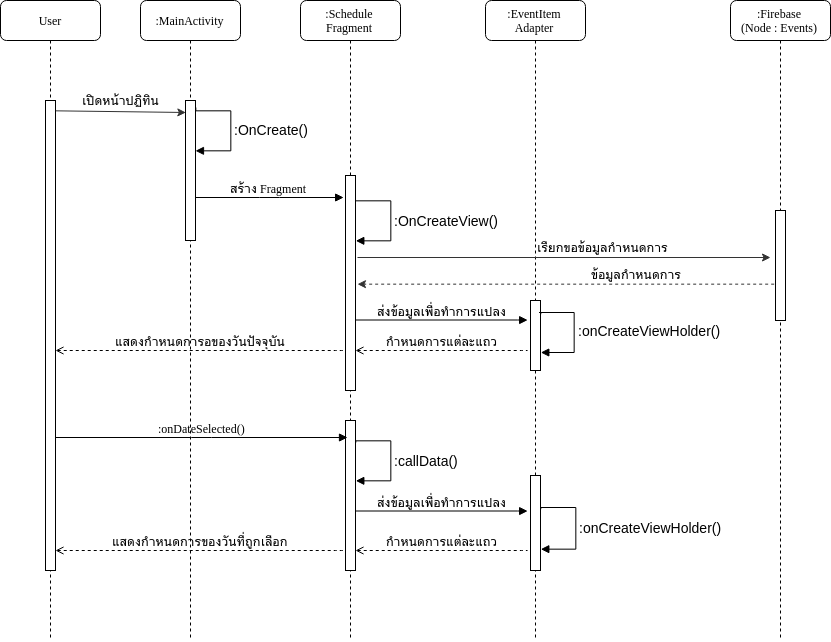
\includegraphics[width=0.8\columnwidth]
		{Figures/3/Sequence/calendar}
		\caption{Sequence Diagram การแสดงปฏิทินกำหนดการ}
		\label{Fig:Sequence-calendar}
	\end{figure}
	\end{sidewaysfigure}
	\newpage
	จากภาพที่ \ref{Fig:Sequence-calendar} สามารถอธิบายแผนภาพ Sequence Diagram แสดงปฏิทินกำหนดการ ได้ดังนี้ เมื่อ
	ผู้ใช้เปิดโปรแกรมระบบจะเรียกใช้เมธอด onCreate() ที่คลาส MainActivity ระบบจะทำการสร้าง
	Fragment ขึ้นมาโดยใช้เมธอด onCreate() ที่คลาส ScheduleFragment เมื่อ ScheduleFragment ถูกติดตั้งบน MainActivity เมธอด callData() จะสืบค้นข้อมูลกำหนดการของวันปัจจุบันจากฐานข้อมูลบน Firebase FireStore และส่งข้อมูลที่ได้ไปแปลงที่คลาส Schedule-ItemAdapter โดยมีการคืนค่าเป็นข้อมูลกำหนดการแต่ละแถวและในขั้นตอนสุดท้ายคลาส Schedule-Fragment จะทำการแสดงรายการกำหนดการวันปัจจุบันออกทางหน้าจอ หากผู้ใช้มีการกดเลือกวันที่ที่ต้องการทราบกำหนดการจากปฏิทินคลาส ScheduleFragment จะทำการเรียกใช้ callData() อีกครั้งโดยสืบค้นข้อมูลกำหนดการของวันที่ถูกเลือกจากฐานข้อมูลบน Firebase FireStore และส่งข้อมูลที่ได้ไปแปลงที่คลาส ScheduleItemAdapter โดยมีการคืนค่าเป็นข้อมูลแต่กำหนดการละแถวและในขั้นตอนสุดท้ายคลาส ScheduleFragment จะทำการแสดงรายการกำหนดการวันที่ผู้ใช้เลือกออกทางหน้าจอ

	\begin{sidewaysfigure}
	\begin{figure}[H]
		\centering
		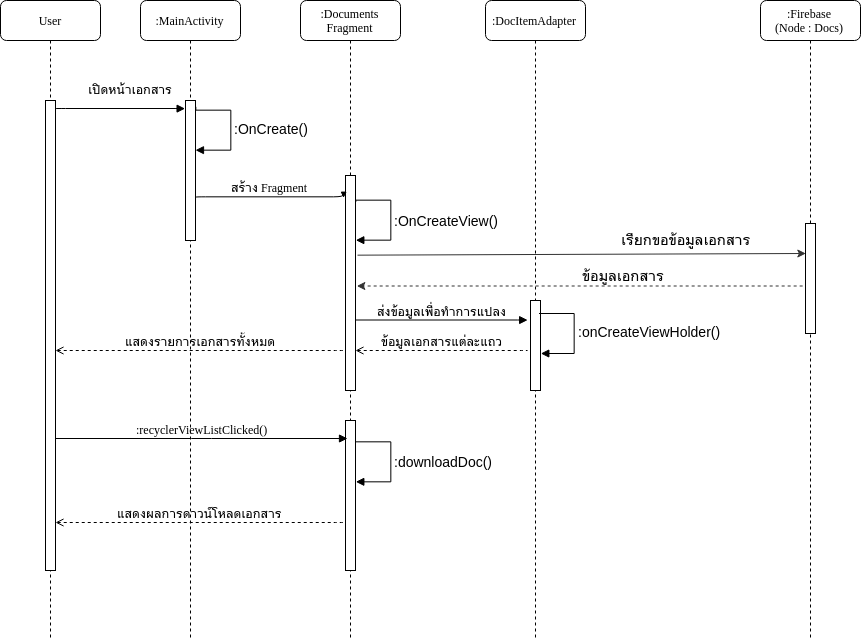
\includegraphics[width=0.8\columnwidth]
		{Figures/3/Sequence/doc}
		\caption{Sequence Diagram การแสดงดาวน์โหลดเอกสาร}
		\label{Fig:Sequence-doc}
	\end{figure}
	\end{sidewaysfigure}
	\newpage
	จากภาพที่ \ref{Fig:Sequence-doc} สามารถอธิบายแผนภาพ Sequence Diagram แสดงดาวน์โหลดเอกสาร ได้ดังนี้ เมื่อผู้ใช้เปิดโปรแกรมระบบจะเรียกใช้เมธอด onCreate() ที่คลาส MainActivity ระบบจะทำการสร้าง
	Fragment ขึ้นมาโดยใช้เมธอด onCreate() ที่คลาส DocumentsFragment เมื่อ DocumentsFragment ถูกติดตั้งบน MainActivity เมธอด initInstances() จะสืบค้นข้อมูลเอกสารทั้งหมดจากฐานข้อมูลบน Firebase FireStore และส่งข้อมูลที่ได้ไปแปลงที่คลาส DocItem-Adapter โดยมีการคืนค่าเป็นข้อมูลเอกสารแต่ละแถวและในขั้นตอนสุดท้ายคลาส Documents-Fragment จะทำการแสดงรายการกำหนดการวันปัจจุบันออกทางหน้าจอ

	\begin{sidewaysfigure}
	\begin{figure}[H]
		\centering
		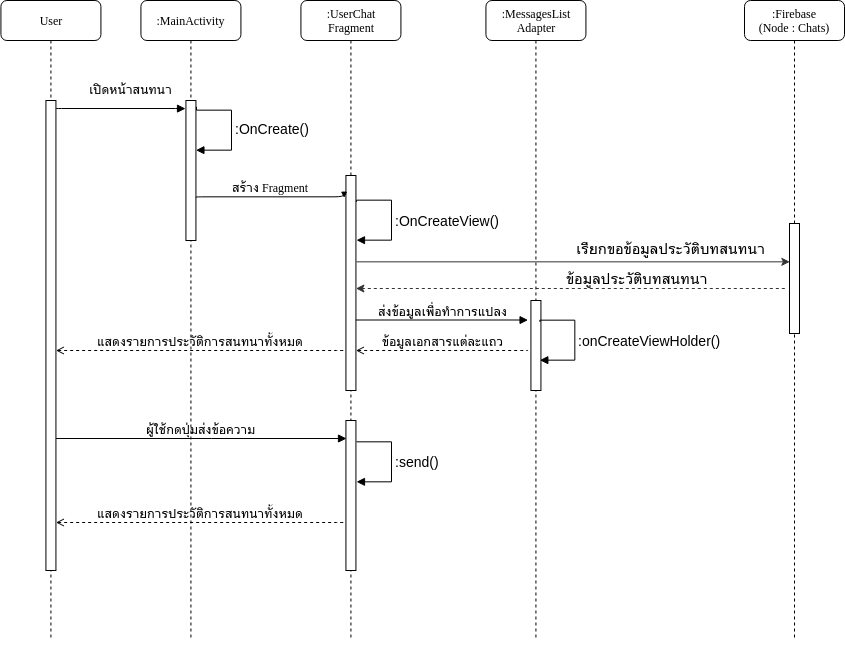
\includegraphics[width=0.8\columnwidth]
		{Figures/3/Sequence/chat}
		\caption{Sequence Diagram การแสดงบทสนทนา}
		\label{Fig:Sequence-chat}
	\end{figure}
	\end{sidewaysfigure}
	\newpage
	จากภาพที่ \ref{Fig:Sequence-chat} สามารถอธิบายแผนภาพ Sequence Diagram แสดงการสนทานา ได้ดังนี้ เมื่อผู้ใช้เปิดโปรแกรมระบบจะเรียกใช้เมธอด onCreate() ที่คลาส MainActivity ระบบจะทำการสร้าง
	Fragment ขึ้นมาโดยใช้เมธอด onCreate() ที่คลาส UserChatFragment เมื่อ UserChatFrag-ment ถูกติดตั้งบน MainActivity เมธอด getMessage() จะสืบค้นข้อมูลประวัติการสนทนาของผู้ใช้คนปัจจุบันทั้งหมดจากฐานข้อมูลบน Firebase FireStore และส่งข้อมูลที่ได้ไปแปลงที่คลาส MessagesListAdapter โดยมีการคืนค่าเป็นข้อมูลรายการประวัติการสนทนาทั้งหมดและในขั้นตอนสุดท้ายคลาส User-ChatFragment จะทำการแสดงรายการประวัติการสนทนาทั้งหมดออกทางหน้าจอ เมื่อผู้ใช้พิมพ์ข้อความและกดปุ่มส่งระบบจะเรียกให้เมธอด send() เพื่อทำการบันทึกข้อมูลไว้บน Firebase FireStore และทำการแสดงข้อมูลรายการประวัติการสนทนาทั้งหมดที่ถูกอัพเดท

	\begin{sidewaysfigure}
	\begin{figure}[H]
		\centering
		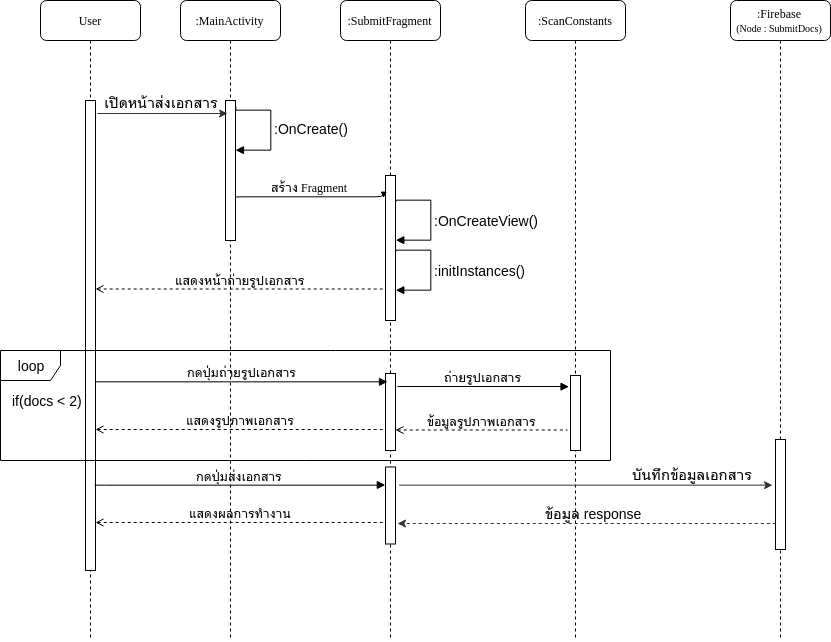
\includegraphics[width=0.8\columnwidth]
		{Figures/3/Sequence/submit}
		\caption{Sequence Diagram แสดงส่งเอกสารตรวจสอบ}
		\label{Fig:Sequence-submit}
	\end{figure}
	\end{sidewaysfigure}
	\newpage
	จากภาพที่ \ref{Fig:Sequence-submit} สามารถอธิบายแผนภาพ Sequence Diagram แสดงส่งเอกสารตรวจสอบ ได้ดังนี้ เมื่อผู้ใช้เปิดโปรแกรมระบบจะเรียกใช้เมธอด onCreate() ที่คลาส MainActivity ระบบจะทำการสร้าง
	Fragment ขึ้นมาโดยใช้เมธอด onCreate() ที่คลาส SubmitFragment เมื่อ Submit-Fragment ถูกติดตั้งบน MainActivity เมธอด initInstances() จะถูกเรียกเพื่อสร้างหน้าจอแสงดผลเมื่อผู้ใช้กดปุ่มถ่ายรูประบบจะเรียกใช้ไลบรารี่ ScanConstants เพื่อถ่ายภาพเอกสารและรอให้ผู้ใช้ถ่ายครบทั้งสองแผ่นจึงจะแสดงปุ่มกดส่งเอกสารเพื่อตรวจสอบ
\newpage	 
	
\section{โครงสร้างฐานข้อมูลไฟร์เบส(Firebase Database Stucture)}
Firebase Database นั้นเป็น Database แบบ NoSQL และเป็น JSON database ที่มีโครงสร้างที่เป็น Key และ Value จัดเก็บข้อมูลในลักษณะโหนด หากต้องการเรียกงานจะเรียกใช้โดย
การท่องไปยังโหนดที่ต้องการ ส่วนประกอบสัญลักษณ์ที่ใช้ในการเขียนโครงสร้างฐานข้อมูลแบบ Firebase
แสดงดังตารางที่ \ref{tab:DB}

\begin{table}[H]
	\centering
	\caption{สัญลักษณ์ของโครงสร้างฐานข้อมูลแบบ Firebase}
	\label{tab:DB}
	\begin{tabular}{| c	| p{10cm} |}
		\hline
		\textbf{สัญลักษณ์} & \multicolumn{1}{c|}{\textbf{คำอธิบาย}} \\ \hline
		\raisebox{-\totalheight}{
\includegraphics[width=0.1\textwidth]{Figures/3/DB/dbroot}}
		& \setstretch{1.5} {Database เป็นการเรียกชื่อแทนโหนด(Node)บนสุดที่ใช้ในการเก็บข้อมูล} \\ \hline
		\raisebox{-\totalheight}{
\includegraphics[width=0.1\textwidth]{Figures/3/DB/dbcollection}}
		& \setstretch{1.5} {Collection เป็นการเรียกชื่อแทนของการเก็บหลาย ๆ เอกสารไว้ด้วยกัน} \\ \hline
		\raisebox{-\totalheight}{
\includegraphics[width=0.1\textwidth]{Figures/3/DB/dbdoc}}
		& \setstretch{1.5} {Document เป็นการเรียกชื่อแทนหน่วยการเก็บของข้อมูลใน Cloud Firestore ภายในจะประกอบไปด้วย ชื่อของ Document  ชื่อของคีย์ (key) และ ค่าข้อมูล (value) โดยชื่อของ Document ห้ามซ้ำกัน ซึ่งใน Cloud Firestore สามารถระบุประเภทของข้อมูลได้ 9 ประเภทได้แก่ boolean, number, string, geo point, timestamp, array, object, reference และ null} \\ \hline
	\end{tabular}
\end{table}
	\begin{figure}[H]
	\centering
	
\includegraphics[width=0.7\columnwidth]
	{Figures/3/DB/DB1}
	\caption{โครงสร้างฐานข้อมูลแบบ Firebase}
	\label{Fig:DB1}
	\end{figure}

	\begin{figure}[H]
	\centering
	
\includegraphics[width=0.9\columnwidth]
	{Figures/3/DB/DB2}
	\caption{โครงสร้างฐานข้อมูลแบบ Firebase(ต่อ)}
	\label{Fig:DB2}
\end{figure}
	\begin{figure}[H]
	\centering
	
\includegraphics[width=0.55\columnwidth]
	{Figures/3/DB/DB3}
	\caption{โครงสร้างฐานข้อมูลแบบ Firebase(ต่อ)}
	\label{Fig:DB3}
\end{figure}
	\begin{figure}[H]
	\centering
	
\includegraphics[width=0.7\columnwidth]
	{Figures/3/DB/DB4}
	\caption{โครงสร้างฐานข้อมูลแบบ Firebase(ต่อ)}
	\label{Fig:DB4}
\end{figure}

\newpage
จากรูที่ \ref{Fig:DB1}-\ref{Fig:DB4} สามารถอธิบายโครงสร้างของข้อมูลได้ดังนี้
\begin{figure}[H]
\centering

\includegraphics[width=0.5\columnwidth]
{Figures/3/DB/nodePost}
\caption{โหนดเก็บข้อมูลประกาศ}
\label{Fig:DB4}
\end{figure}
\begin{table}[H]
	\centering
	\caption{อธิบายโหนดที่ใช้เก็บข้อมูลประกาศ}
	\label{my-label1}
	\begin{tabular}{|c|p{10cm}|}
		\hline
		\multicolumn{1}{|c|}{\textbf{Key}} & \multicolumn{1}{c|}{\textbf{คำอธิบาย}} \\ \hline
		Posts & โหนดสำหรับเก็บข้อมูลประกาศทั้งหมด \\ \hline
		Post &  สำหรับเก็บข้อมูลแต่ละประกาศ \\ \hline
		title & สำหรับเก็บชื่อหัวข้อประกาศ \\ \hline
		description & สำหรับเก็บรายละเอียดประกาศ  \\ \hline
		collection & สำหรับเก็บประเภทของประกาศได้แก่ สาธารณะและเฉพาะบุคคล \\ \hline
		fileURL & สำหรับเก็บ url ของเอกสารแนบประกาศ \\ \hline
		id & สำหรับเก็บรหัสของประกาศ \\ \hline
		time & สำหรับเก็บเวลาที่ประกาศ \\ \hline
	\end{tabular}
\end{table}

\newpage
\begin{figure}[H]
	\centering
	
\includegraphics[width=0.5\columnwidth]
	{Figures/3/DB/nodeDoc}
	\caption{โหนดเก็บข้อมูลเอกสารที่เกี่ยวข้อง}
	\label{Fig:DB4}
\end{figure}
\begin{table}[H]
	\centering
	\caption{อธิบายโหนดที่ใช้เก็บข้อมูลเอกสารที่เกี่ยวข้อง}
	\label{my-label1}
	\begin{tabular}{|c|p{10cm}|}
		\hline
		\multicolumn{1}{|c|}{\textbf{Key}} & \multicolumn{1}{c|}{\textbf{คำอธิบาย}} \\ \hline
		Docs & โหนดสำหรับเก็บข้อมูลของเอกสารที่เกี่ยวข้องทั้งหมด \\ \hline
		Doc &  สำหรับเก็บข้อมูลเอกสารแต่ละฉบับ \\ \hline
		title & สำหรับเก็บชื่อหัวเรื่องของเอกสาร \\ \hline
		description & สำหรับเก็บรายละเอียดของเอกสาร \\ \hline
		fileType & สำหรับนามสกุลไฟล์เอกสาร เช่น .pdf .png เป็นต้น \\ \hline
		fileURL & สำหรับเก็บ url ของเอกสาร\\ \hline
		time & สำหรับเก็บเวลาที่ถูกอัพโหลดเข้าสู่ระบบโดยเจ้าหน้าที่\\ \hline
	\end{tabular}
\end{table}

\newpage
\begin{figure}[H]
	\centering
	
\includegraphics[width=0.4\columnwidth]
	{Figures/3/DB/nodeChat}
	\caption{โหนดเก็บข้อมูลประวัติการสนทนา}
	\label{Fig:DB4}
\end{figure}
\begin{table}[H]
	\centering
	\caption{อธิบายโหนดที่ใช้เก็บข้อมูลประวัติการสนทนา}
	\label{my-label1}
	\begin{tabular}{|c|p{10cm}|}
		\hline
		\multicolumn{1}{|c|}{\textbf{Key}} & \multicolumn{1}{c|}{\textbf{คำอธิบาย}} \\ \hline
		Chats & โหนดสำหรับเก็บข้อมูลประวัติการสนทนาทั้งหมด \\ \hline
		User\_id &  สำหรับเก็บประวัติการสนทนาของผู้ใช้แต่ละคน \\ \hline
		Messages & สำหรับเก็บประวัติการสนทนาทั้งหมดของผู้ใช้ \\ \hline
		Message & สำหรับเก็บข้อมูลของแต่ละข้อความ \\ \hline
		message & สำหรับเก็บข้อความ \\ \hline
		name & สำหรับเก็บชื่อของผู้ส่งข้อความ\\ \hline
		photo & สำหรับเก็บ url รูปภาพของผู้ส่งข้อความ\\ \hline
		senderId & สำหรับเก็บรหัสของผู้ส่งข้อความ\\ \hline
		time & สำหรับเก็บเวลาที่ข้อความถูกส่ง\\ \hline
	\end{tabular}
\end{table}

\newpage
\begin{figure}[H]
	\centering
	
\includegraphics[width=0.5\columnwidth]
	{Figures/3/DB/nodeEvent}
	\caption{โหนดเก็บข้อมูลกำหนดการ}
	\label{Fig:DB4}
\end{figure}
\begin{table}[H]
	\centering
	\caption{อธิบายโหนดที่ใช้เก็บข้อมูลกำหนดการ}
	\label{my-label1}
	\begin{tabular}{|c|p{10cm}|}
		\hline
		\multicolumn{1}{|c|}{\textbf{Key}} & \multicolumn{1}{c|}{\textbf{คำอธิบาย}} \\ \hline
		Events & โหนดสำหรับเก็บข้อมูลของกำหนดการทั้งหมด \\ \hline
		Event & สำหรับเก็บข้อมูลของแต่ละกำหนดการ \\ \hline
		title & สำหรับเก็บชื่อหัวข้อของกำหนดการ \\ \hline
		description & สำหรับเก็บรายละเอียดของกำหนดการ\\ \hline
		time & สำหรับเก็บเวลาของกำหนดการ\\ \hline
	\end{tabular}
\end{table}

\newpage
\begin{figure}[H]
	\centering
	
\includegraphics[width=0.4\columnwidth]
	{Figures/3/DB/nodeReq}
	\caption{โหนดเก็บข้อมูลการยื่นสำเนาเอกสารเพื่อตรวจสอบของนักศึกษา}
	\label{Fig:DB4}
\end{figure}
\begin{table}[H]
	\centering
	\caption{อธิบายโหนดที่ใช้เก็บข้อมูลการยื่นสำเนาเอกสารเพื่อตรวจสอบของนักศึกษา}
	\label{my-label1}
	\begin{tabular}{|c|p{10cm}|}
		\hline
		\multicolumn{1}{|c|}{\textbf{Key}} & \multicolumn{1}{c|}{\textbf{คำอธิบาย}} \\ \hline
		RusetSubmitDocs & โหนดสำหรับเก็บข้อมูลการยื่นสำเนาเอกสารเพื่อตรวจสอบของนักศึกษาทั้งหมด \\ \hline
		User\_id & สำหรับเก็บข้อมูลของแต่ละสำเนาเอกสารของนักศึกษาแต่ละคน \\ \hline
		doc2 & สำหรับเก็บ url ของภาพถ่ายสำเนาเอกสารฉบับที่ 1\\ \hline
		doc2 & สำหรับเก็บ url ของภาพถ่ายสำเนาเอกสารฉบับที่ 2\\ \hline
		status & สำหรับเก็บผลการตรวจสอบของเจ้าหน้าที่ \\ \hline
		time & สำหรับเก็บเวลาที่สำเนาเอกสารถูกเพิ่มเข้าสู่ระบบ \\ \hline
	\end{tabular}
\end{table}

\newpage
\begin{figure}[H]
	\centering
	
\includegraphics[width=0.35\columnwidth]
	{Figures/3/DB/nodeUser}
	\caption{โหนดเก็บข้อมูลของนักศึกษา}
	\label{Fig:DB4}
\end{figure}
\begin{table}[H]
	\centering
	\caption{อธิบายโหนดที่ใช้เก็บข้อมูลของนักศึกษา}
	\label{my-label1}
	\begin{tabular}{|c|p{10cm}|}
		\hline
		\multicolumn{1}{|c|}{\textbf{Key}} & \multicolumn{1}{c|}{\textbf{คำอธิบาย}} \\ \hline
		Users & โหนดสำหรับเก็บข้อมูลของนักศึกษา \\ \hline
		User\_id & สำหรับเก็บข้อมูลของนักศึกษาแต่ละคน \\ \hline
		depart & สำหรับเก็บภาควิชาของนักศึกษา\\ \hline
		major & สำหรับเก็บสาขาของนักศึกษา\\ \hline
		sid & สำหรับเก็บรหัสประจำตัวนักศึกษา \\ \hline
		name & สำหรับเก็บชื่อของนักศึกษา \\ \hline
		year & สำหรับเก็บชั้นปีของนักศึกษา \\ \hline
		lastChat & สำหรับเก็บเวลาที่สนทนากับเจ้าหน้าที่ล่าสุด \\ \hline
		photoUrl & สำหรับเก็บ url รูปภาพโปรไฟล์ (Profile) \\ \hline
	\end{tabular}
\end{table}

\newpage
\begin{figure}[H]
	\centering
	
\includegraphics[width=0.5\columnwidth]
	{Figures/3/DB/nodeQueue}
	\caption{โหนดเก็บข้อมูลการจองคิวของนักศึกษา}
	\label{Fig:DB4}
\end{figure}
\begin{table}[H]
	\centering
	\caption{อธิบายโหนดที่ใช้เก็บข้อมูลการจองคิวของนักศึกษา}
	\label{my-label1}
	\begin{tabular}{|c|p{10cm}|}
		\hline
		\multicolumn{1}{|c|}{\textbf{Key}} & \multicolumn{1}{c|}{\textbf{คำอธิบาย}} \\ \hline
		Queue & โหนดสำหรับเก็บข้อมูลการจองคิวของนักศึกษาทั้งหมด \\ \hline
		q\_id &  สำหรับเก็บข้อมูลของการจองคิวแต่ละครั้งที่เปิดจองคิว \\ \hline
		Date &  สำหรับเก็บวันที่สำหรับส่งเอกสาร\\ \hline
		Time &  สำหรับเก็บรายชื่อของนักศึกษาที่ทำการจองคิวในส่งเอกสารเวลานั้น ๆ\\ \hline
		User\_id & สำหรับเก็บรหัสของนักศึกษา \\ \hline
		title & สำหรับเก็บชื่อหัวเรื่องกำหนดการการจองคิว \\ \hline
		studentPerHr & สำหรับเก็บจำนวนนักศึกษาต่อชั่วโมง \\ \hline
	\end{tabular}
\end{table}

\newpagedr
\begin{figure}[H]
	\centering
	
\includegraphics[width=0.4\columnwidth]
	{Figures/3/DB/nodeFaq}
	\caption{โหนดเก็บข้อมูลคำถามที่พบบ่อย}
	\label{Fig:DB4}
\end{figure}
\begin{table}[H]
	\centering
	\caption{อธิบายโหนดที่ใช้เก็บข้อมูลคำถามที่พบบ่อย}
	\label{my-label1}
	\begin{tabular}{|c|p{10cm}|}
		\hline
		\multicolumn{1}{|c|}{\textbf{Key}} & \multicolumn{1}{c|}{\textbf{คำอธิบาย}} \\ \hline
		Queue & โหนดสำหรับเก็บข้อมูลคำถามที่พบบ่อยทั้งหมด \\ \hline
		Faq\_id & สำหรับเก็บข้อมูลคำถามที่พบบ่อยแต่ละรายการ \\ \hline
		title & สำหรับเก็บคำถาม \\ \hline
		description & สำหรับเก็บคำตอบ \\ \hline
	\end{tabular}
\end{table}
